% !TeX spellcheck = en_US
% !TeX encoding = UTF-8
\documentclass[a4paper]{article}
\usepackage{graphics, graphicx}
\usepackage{fancyvrb, enumerate}
\usepackage{amsmath, amssymb, amscd, amsfonts}
\usepackage{geometry}
\usepackage{multirow}
\usepackage{url}
\usepackage{listings, listing}
\usepackage{color}
\usepackage{mathptmx}
\usepackage[numberedbib]{apacite}
\usepackage[style=iso]{datetime2}
\usepackage{csvsimple, booktabs}
\usepackage[maxfloats=256]{morefloats}
\maxdeadcycles=1000

\geometry
{
    top = 20mm,
    bottom = 20mm,
    left = 20mm,
    right = 20mm
}

\title{Periodontitis}
\author{
    Jaewoong Lee
    \and
    Seunghoon Kim
    \and
    Semin Lee
}
\date{\today}

\begin{document}
   	\maketitle
    \newpage

    \tableofcontents
    \listoftables
    \listoffigures
    \newpage

    \section{Introduction}
        \subsection{Microbiome}
            Microbiome is consist of microbiota, the micro-organisms which live inside and on humans \cite{microbiome1}. Microbiome is also about $10^{13}$ micro-organisms whose which collective genome \cite{microbiome2}.

            \begin{figure}[p]
                \centering
                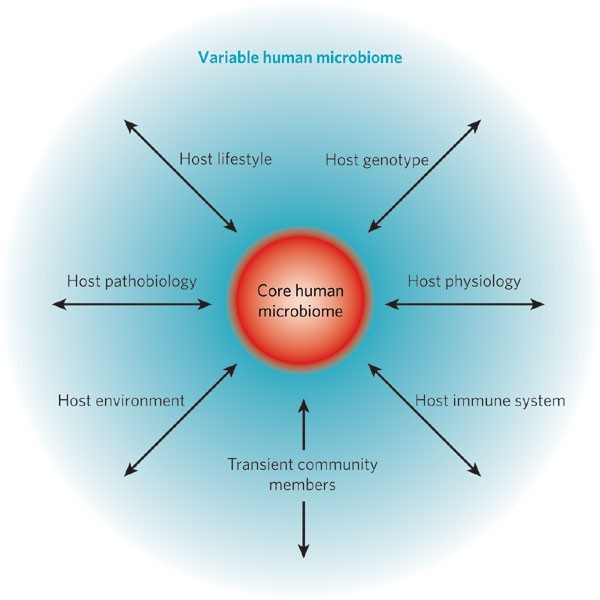
\includegraphics[width=0.5 \linewidth]{figures/microbiome.jpg}
                \caption{Concept of a Core Human Microbiome \protect\cite{microbiome1}}
                \label{fig:microbiome-concept}
            \end{figure}

        \subsection{Ribosomal RNA}
            Ribosomal RNA (rRNA) is well-known as a key to phylogeny \cite{rRNA1}.

        \subsection{16S rRNA Gene Sequencing}

        \subsection{Periodontitis}
            Periodontitis is an inflammatory conditions which effecting periodontium, tissues  which surround and support teeth. Major components of periodontitis are clinical attachment loss and bone loss \cite{periodontitis1}. Previous study found risk factors of periodontitis such as smoking, diabetes, genetic factors and host response \cite{periodontitis2}.

    \section{Materials}
        \subsection{16S rRNA Gene Sequencing}

            \begin{itemize}
                \item 100 Healthy samples
                \item 50 Chronic Early Periodontitis Sample
                \item 50 Chronic Moderate Periodontitis Sample
                \item 50 Chronic Severe Periodontitis Sample
            \end{itemize}

    \section{Methods}
        \subsection{QIIME2 Workflow}
            QIIME2 is a capable, expandable and distributed microbiome analysis package with transparent analysis \cite{qiime1, qiime2}. A theoretic overview of QIIME2 workflow is shown as figure \ref{fig:qiime-workflow}.

            \begin{figure}[p]
                \centering
                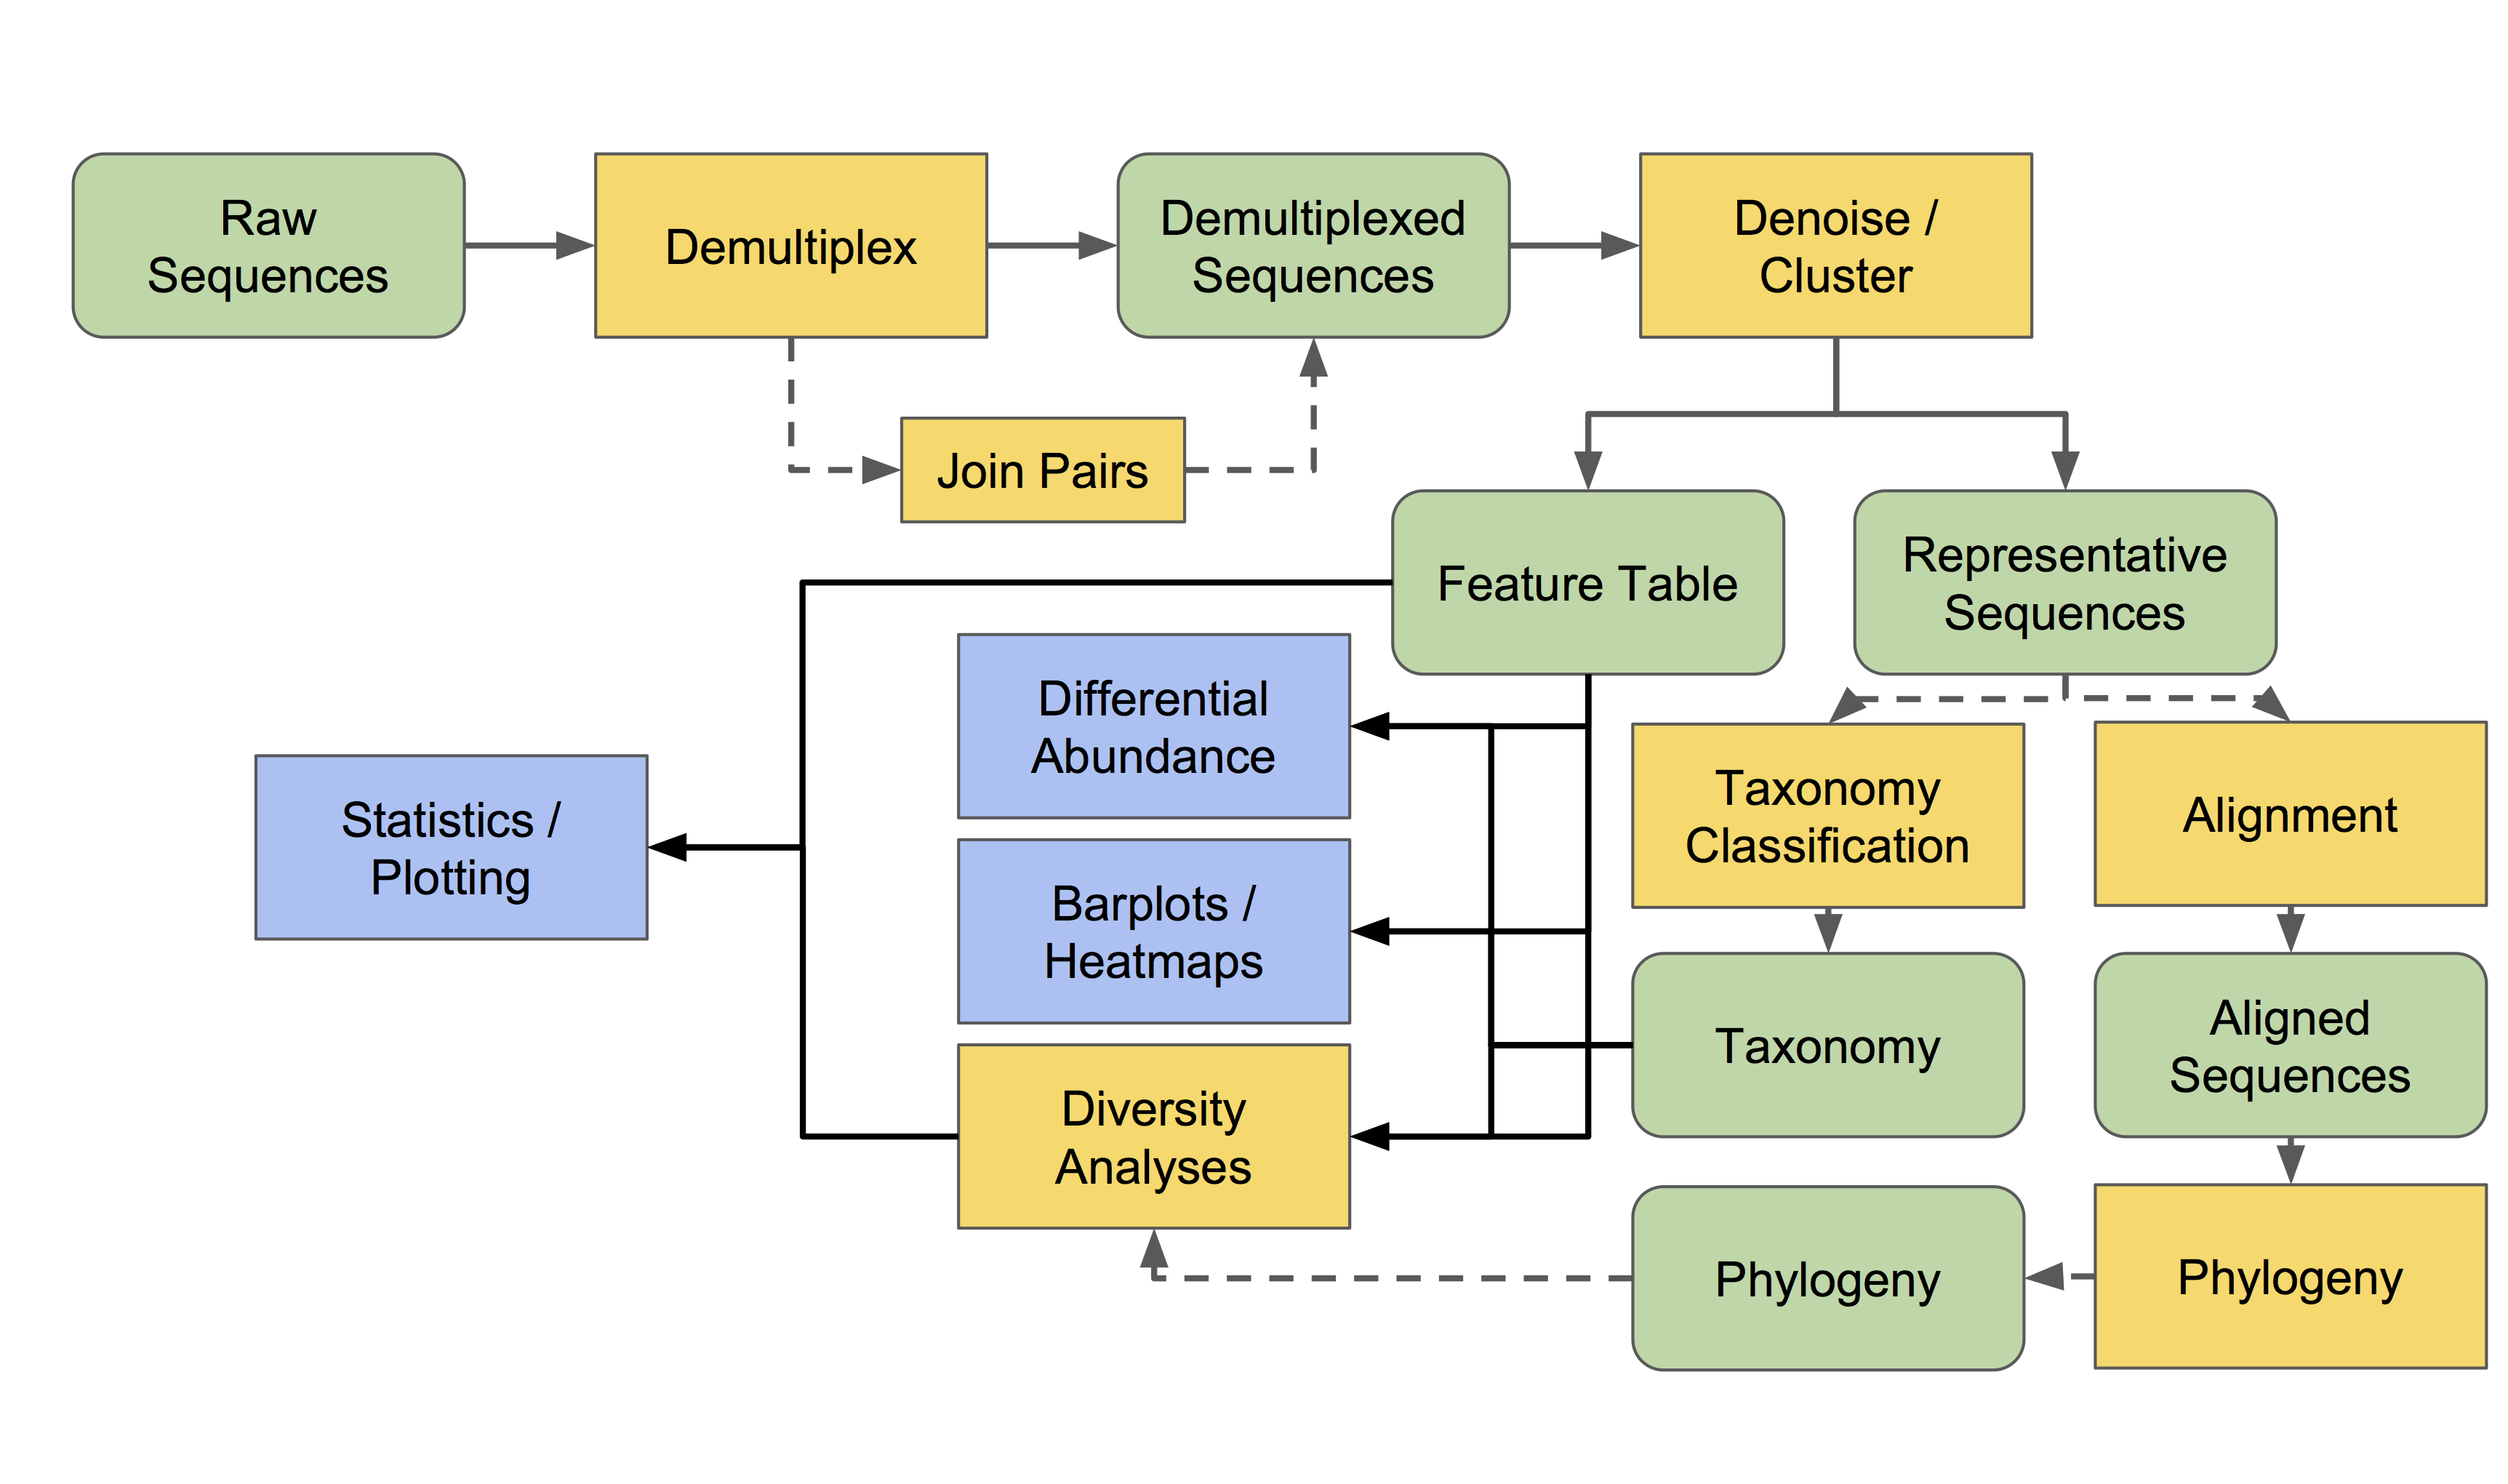
\includegraphics[width=0.8 \linewidth]{figures/qiime.png}
                \caption{A Theoretic Overview of QIIME2 Workflow \protect\cite{qiime1, qiime2}}
                \label{fig:qiime-workflow}
            \end{figure}

            \subsubsection{Denoising techniques}
                There are two denoising techniques provided by QIIME2: DADA2 \cite{DADA1} and Deblur \cite{deblur1}. Major difference between DADA2 and Deblur, as shown as figure \ref{fig:denosing-workflow}, is a strategy, the strategy used to divide as different species. DADA2 uses amplicon sequence variants (ASVs), strictly divides sequences even one-base mismatch. However, Deblur uses operational taxonomic units (OTUs), considers as same sequence when sequences are 97 \% or more matched.

                \begin{figure}[p]
                    \centering
                    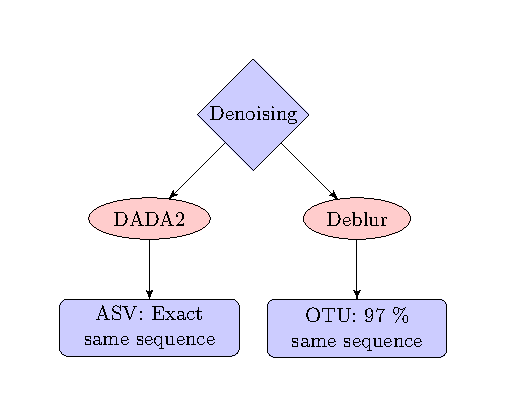
\includegraphics[width=0.5 \linewidth]{figures/denoising/denoising.pdf}
                    \caption{Denoising Techniques which provided by QIIME2}
                    \label{fig:denosing-workflow}
                \end{figure}

            \subsubsection{Taxonomy Classification}
                There are two taxonomy classification databases which provided by QIIME2: Greengenes (GG) \cite{greengenes1} and SILVA \cite{silva1}. Major difference between Greengenes and SILVA is resolution. Resolution of Greengenes is from kingdom to species; however, resolution of SILVA is from domain to genus. Note that a higher accuracy at taxonomic levels above genus level; but accuracy drops at species level \cite{performance1}.

                \begin{figure}[p]
                    \centering
                    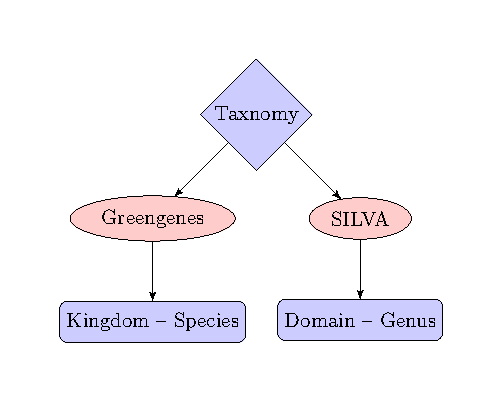
\includegraphics[width=0.5 \linewidth]{figures/taxonomy/taxonomy.pdf}
                    \caption{Taxonomy Classification which provided by QIIME2}
                    \label{fig:taxonomy-workflow}
                \end{figure}

            \subsubsection{Merging Denoising and Taxonomy Classification}
                After denosing and taxonomy classification steps, some different IDs (ASVs or OTUs) have been identified as same taxonomy. In that case, the different IDs will be merged into one taxonomy (Figure \ref{fig:merging}).

                \begin{figure}[p]
                    \centering
                    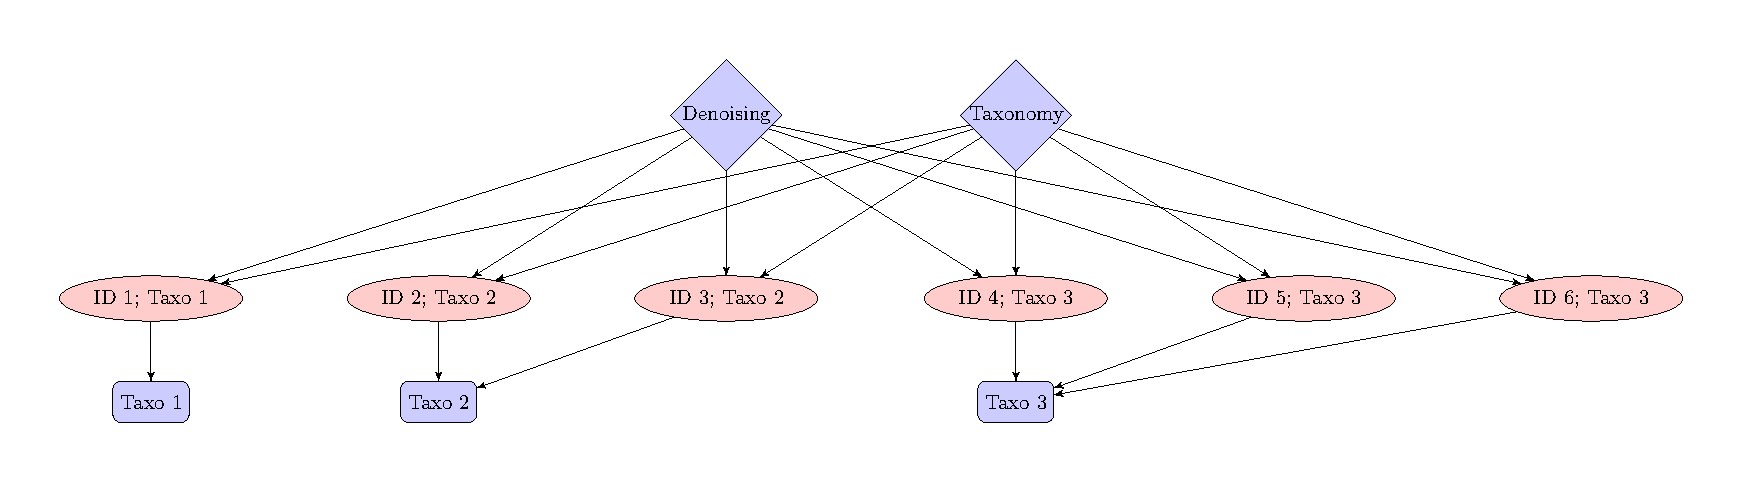
\includegraphics[width=0.8 \linewidth]{figures/Merging/merging.pdf}
                    \caption{Example Diagram for Merging Denoising and Taxonomy Classification}
                    \label{fig:merging}
                \end{figure}

            \subsubsection{Rarefaction}
                Rarefaction is a statistical method of estimating the number of species expected in a random sample which taken from a collection \cite{rarefaction1}. Moreover, rarefaction allows comparisons of the species richness among communities. Thus, rarefaction is a good choice for normalization \cite{rarefaction2}.

            \subsubsection{Alpha-diversity}
                Alpha-diversity is a metric which shows the richness of taxa at a single community. There are four alpha-diversity indices which provided from QIIME2:
                \begin{itemize}
                    \item Evenness index.
                    \item Faith's phylogenetic diversity (Faith PD).
                    \item Observed features.
                    \item Shannon's diversity index.
                \end{itemize}

                Shannon's diversity index shows a quantitative measure of community richness; Observed features, however, is a qualitative measure of community richness. Faith's phylogenetic diversity index indicates a qualitative measure of community richness which assimilates phylogenetic relationship among features. Finally, evenness index, as its name, shows a measure of community evenness.

            \subsubsection{Beta-diversity}
                Beta-diversity is a metric which indicates the taxonomic differentiation between multiple communities. There are four beta-diversity indices which provided from QIIME2:
                \begin{itemize}
                    \item Bray-Curtis distance.
                    \item Jaccard distance.
                    \item Unweighted UniFrac distance.
                    \item Weighted UniFrac distance.
                \end{itemize}

                Bray-Curtis distance shows a quantitative of community dissimilarity; Jaccard distance, however, indicates a qualitative measure of community dissimilarity. UniFrac distances reveal a measure of community dissimilarity which consolidates phylogenetic relationship among features. Difference between unweighted UniFrac distance and weighted UniFrac distance is a qualitative and a quantitative, respectively.

            \subsubsection{ANCOM}
                ANCOM (Analysis of composition of microbiomes) can be used for analyzing the composition of microbiome in multiple populations \cite{ANCOM1}. Example ANCOM volcano plot is shows as figure \ref{fig:ancom-example}. In figure \ref{fig:ancom-example}, two metrics are clearly shown: clr and W. clr stands for centered $\log$ ratio, and W is a count of the number of sub-hypothesis which have passed for given species.

                \begin{figure}[p]
                    \centering
                    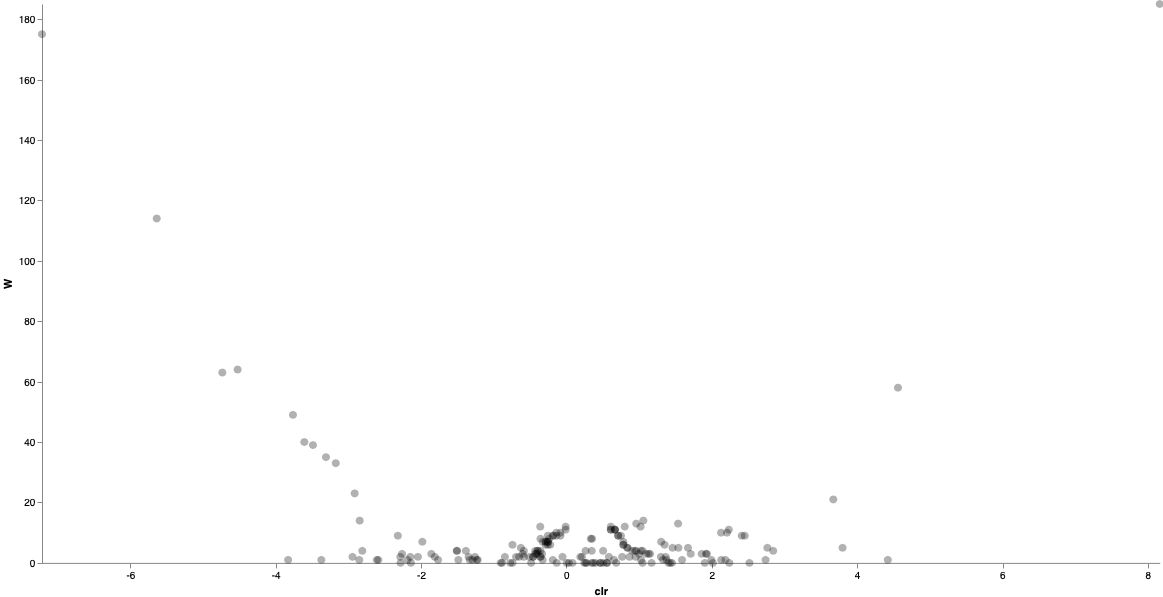
\includegraphics[width=0.8 \linewidth]{figures/ANCOM/example.png}
                    \caption{Example ANCOM Volcano Plot which Provided by QIIME2 \protect\cite{qiime1, qiime2}}
                    \label{fig:ancom-example}
                \end{figure}

        \subsection{Python Packages}
            \subsubsection{Pandas}
                Pandas is a Python package of rich data structures and tools for analyzing with structured data sets \cite{pandas1}.

            \subsubsection{Scikit-learn}
                Scikit-learn grants state-of-the-art implementation of many machine learning algorithms, while controlling an easy-to-use interface tightly integrated the Python code \cite{sklearn1}.

            \subsubsection{Matplotlib}
                Matplotlib is a Python graphics package which used for application development, interactive scripting and publication quality image generation \cite{matplotlib2}. Matplotlib, also, is designed to create simple plots with a few commands \cite{matplotlib1}.

            \subsubsection{Seaborn}
                Seaborn is a Python data visualization package which based on matplotlib, allows a high-level interface for displaying engaging and descriptive statistical graphics \cite{seaborn1}.

        \subsection{t-SNE}
            t-SNE (t-distributed stochastic neighbor embedding) reveals high-dimensional data a location in two-dimensional map \cite{tSNE1}. Figure \ref{fig:tsne-example} is example of t-SNE with hand-writing digits \cite{tSNE1}. In figure \ref{fig:tsne-example}, all 10 digits are grouped into 10 groups clearly; some hand-writings, however, are classified into wrong groups due to their similar shapes, such as 0 and 6.

            \begin{figure}[p]
                \centering
                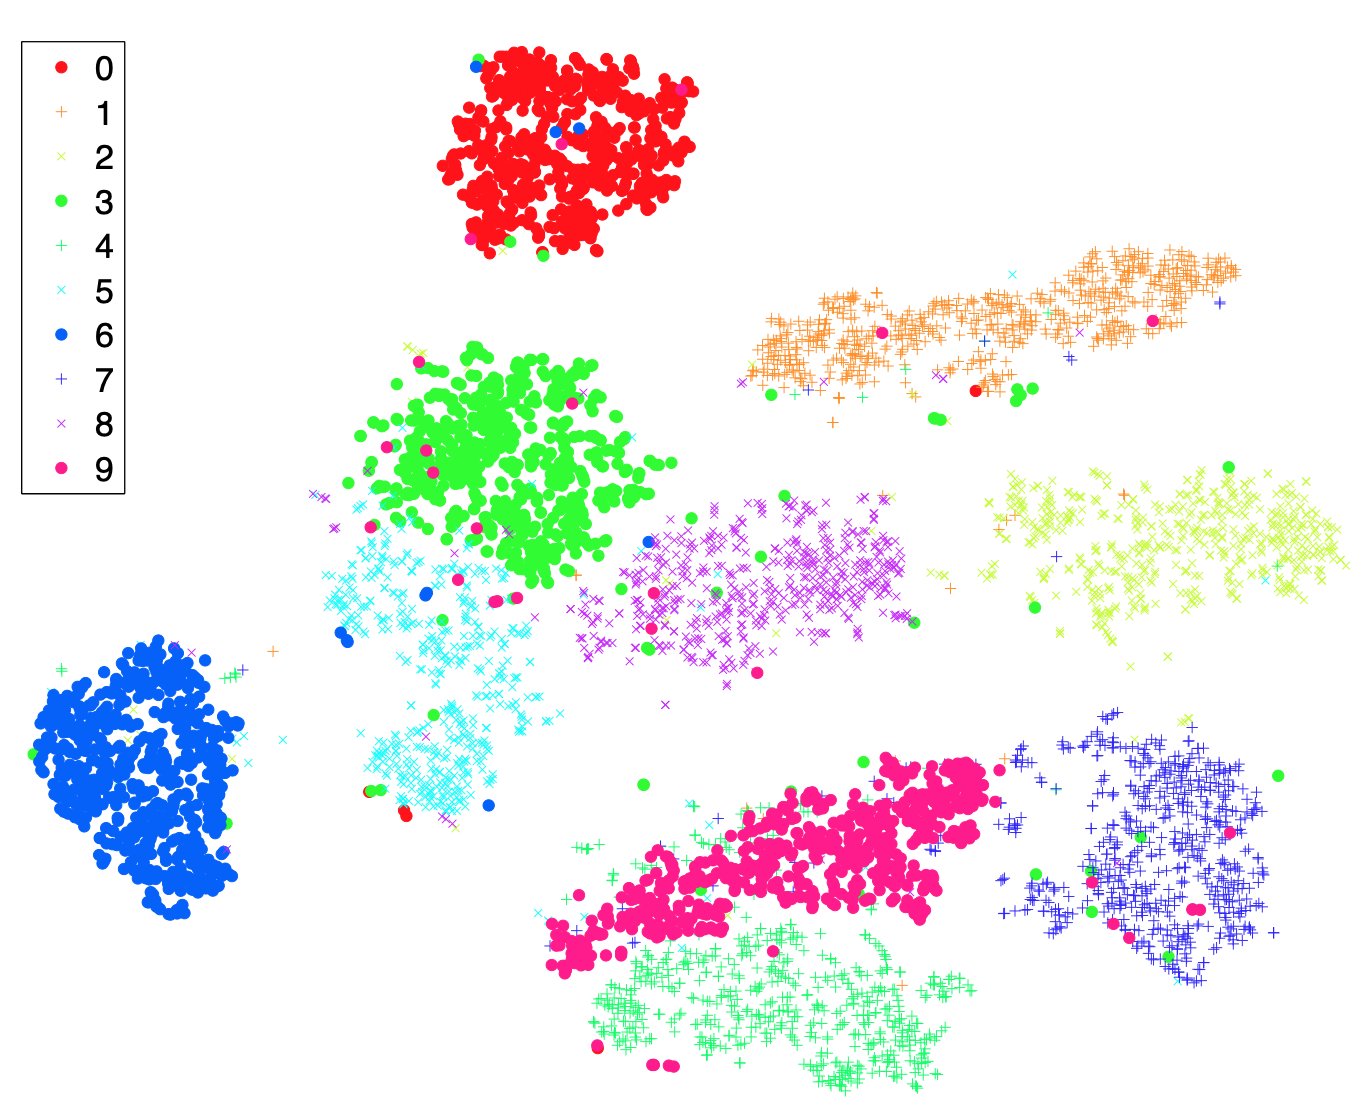
\includegraphics[width=0.4 \linewidth]{figures/tSNE.png}
                \caption{Visualization by t-SNE \protect\cite{tSNE1}}
                \label{fig:tsne-example}
            \end{figure}

        \subsection{Classification}
            In machine learning, Classification is one of supervised learning which identifies a class of a new observation, depends on given information which consist of training observations and their classes.

            In this study, classification will be carried out as figure \ref{fig:classification}; and the third step in figure \ref{fig:classification} is demonstrated in minute detail as figure \ref{fig:deciding-best}. Note that the first step in figure \ref{fig:classification} is optional: due to tables herein-after, such as table\ref{tb:alpha-evenness-dada2}, show that no statistically significant differences between healthy samples and early periodontitis samples and between moderate periodontitis samples and severe periodontitis samples.

            Moreover, in this study, followed classification algorithms are used:
            \begin{itemize}
                \item RandomForest Classification Algorithm \cite{RandomForest1, sklearn1}
            \end{itemize}

            Moreover, evaluations of classification algorithm are carried out with derivations from confusion matrix as table \ref{tb:confusion-matrix}:

            \begin{itemize}
                \item Accuracy (ACC) $ = \frac{TP + TN}{TP + TN + FP + FN}$
                \item Balanced Accuracy (BA) $ = \frac{TP}{2 \times (TP + FN)} + \frac{TN}{2 \times (TN + FP)}$
                \item Sensitivity (SEN) $ = \frac{TP}{TP + FN}$
                \item Specificity (SPE) $ = \frac{TN}{TN + FP}$
                \item Precision (PRE) $ = \frac{TP}{TP + FP}$
            \end{itemize}

            \begin{table}[p]
                \centering
                \caption{Confusion Matrix}
                \label{tb:confusion-matrix}
                \begin{tabular}{c|c|cc}
                    \multicolumn{2}{c|}{\multirow{2}{*}{}} & \multicolumn{2}{c}{Actual Class} \\ \cline{3-4}
                    \multicolumn{2}{c|}{} & Positive & Negative \\ \hline
                    \multirow{2}{*}{Predicted Class} & Positive & True Positive (TP) & False Positive (FP) \\
                    & Negative & False Negative (FN) & True Negative (TN)
                \end{tabular}
            \end{table}

            \begin{figure}[p]
                \centering
                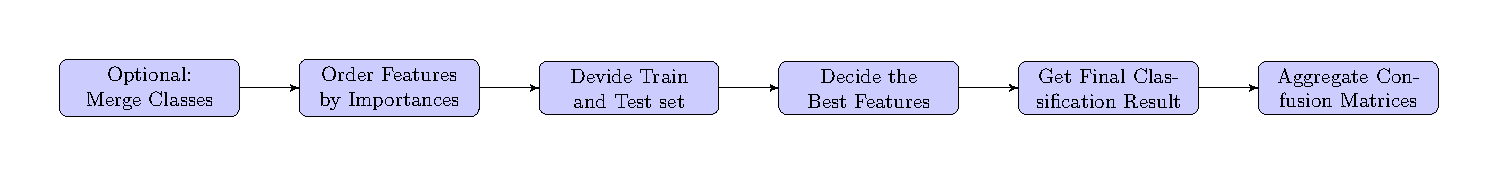
\includegraphics[width=0.8 \linewidth]{figures/Classifier/classifier.pdf}
                \caption{Workflow of Classification}
                \label{fig:classification}
            \end{figure}

            \begin{figure}[p]
                \centering
                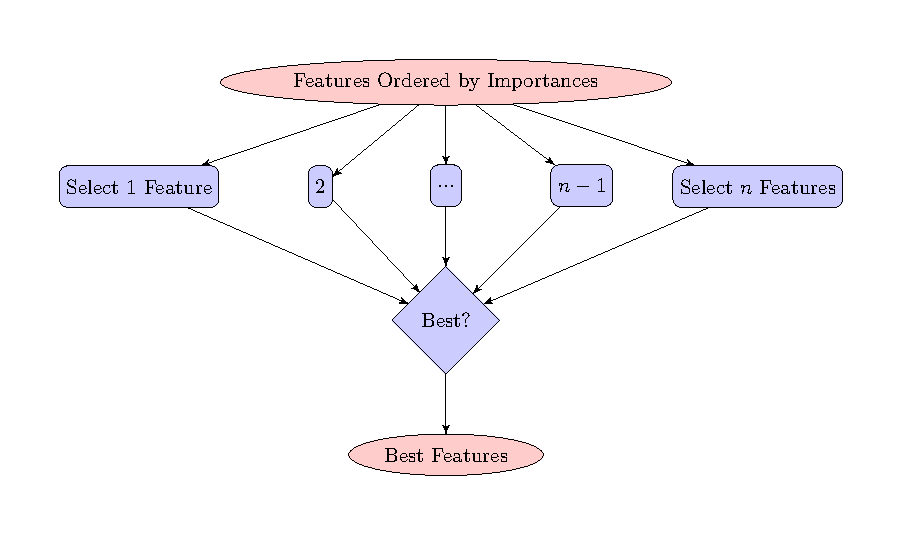
\includegraphics[width=0.6 \linewidth]{figures/Classifier/best.pdf}
                \caption{Deciding the Best Features}
                \label{fig:deciding-best}
            \end{figure}

    \section{Results}
        \subsection{Quality Filter}
            Longer sequences have more fallen sequence quality than shorter. Thus, sequences which longer than threshold should be trimmed out due to their low quality. However, gold-standard strategy for deciding the threshold does not exist; the threshold is set as longest sequence length which have half of sequences have greater than 30 quality score. Hence, sequence quality plot is shown as figure \ref{fig:sequence-quality}; trimmed length in forward reads is 300, and trimmed length in reverse reads is 265.

            \begin{figure}[p]
                \centering
                $\begin{array}{cc}
                    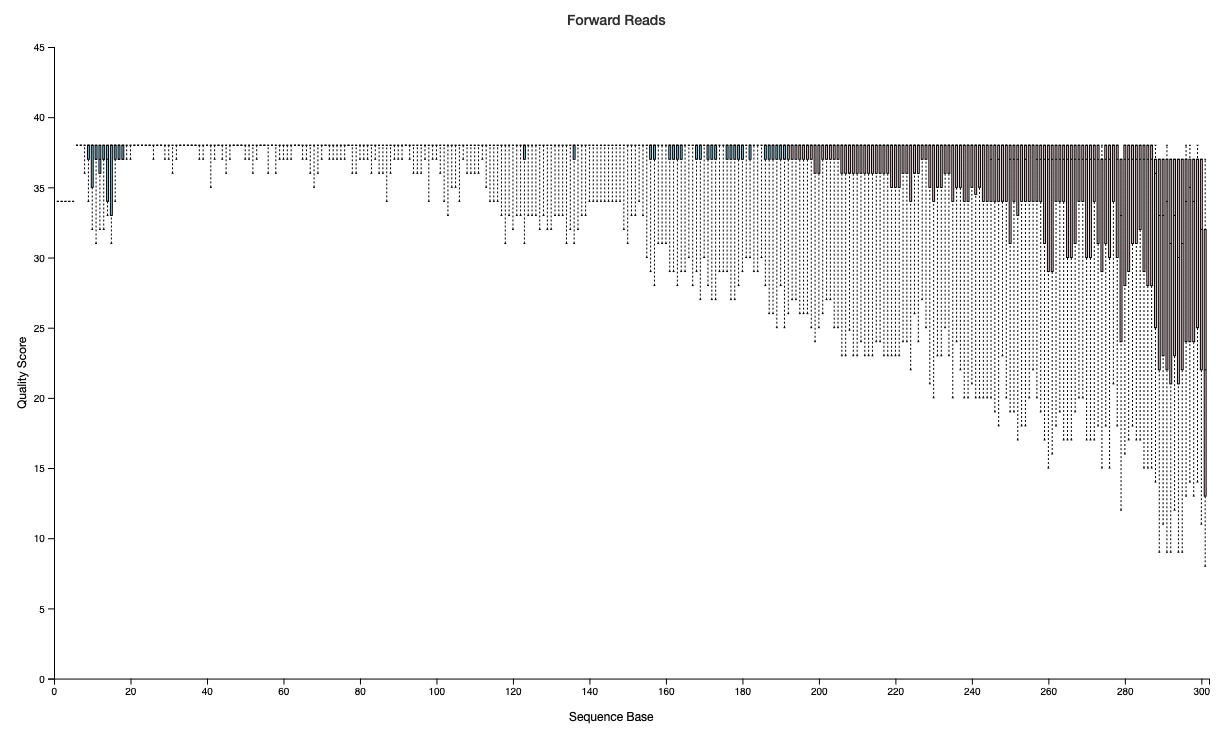
\includegraphics[width=0.4 \linewidth]{figures/QualityFilter/Forward.png}
                    &
                    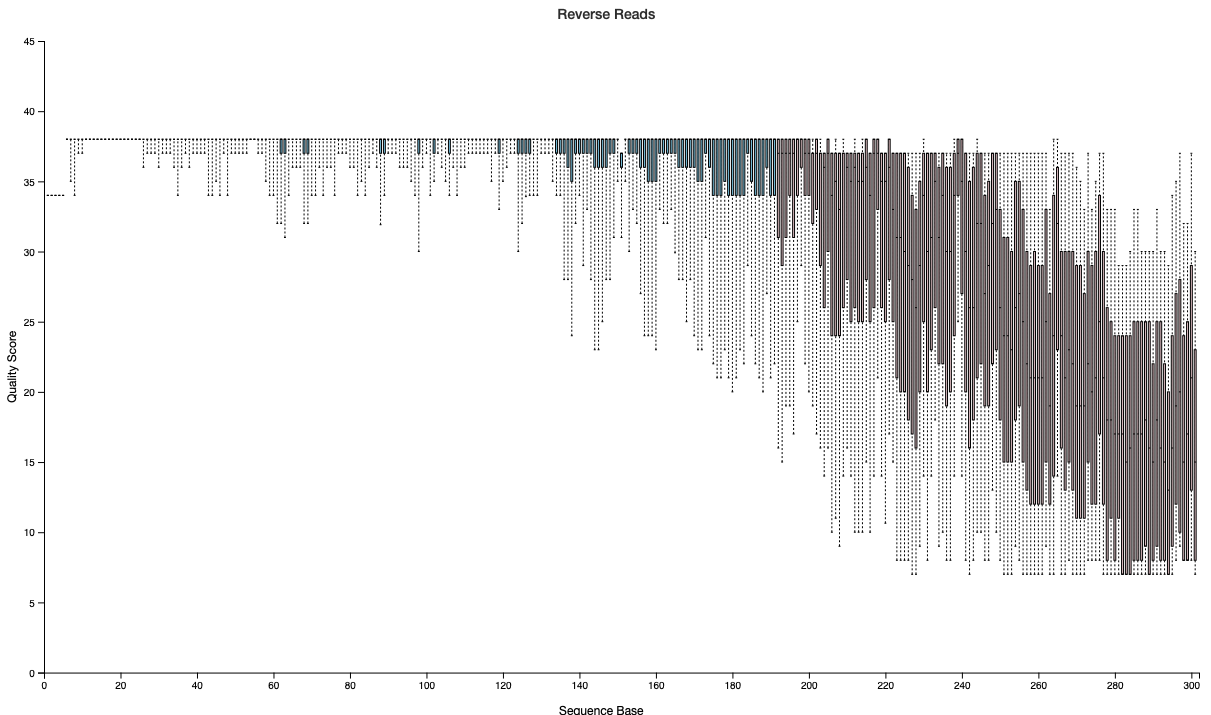
\includegraphics[width=0.4 \linewidth]{figures/QualityFilter/Reverse.png}
                    \\
                    \mbox{(a) Forward Reads} & \mbox{(b) Reverse Reads} \\
                \end{array}$
                \caption{Sequence Quality Plot}
                \label{fig:sequence-quality}
            \end{figure}

        \subsection{Rarefaction}
            Sampling depth should be decided for rarefaction. Gold-standard method for determining sampling depth is minimum frequency in the samples. Hence, sampling depth with DADA2 is 3786 (Figure \ref{fig:frequency-sample-dada2}), and sampling depth with Deblur is 7253 (Figure \ref{fig:frequency-sample-deblur}).

            \begin{figure}[p]
                \centering
                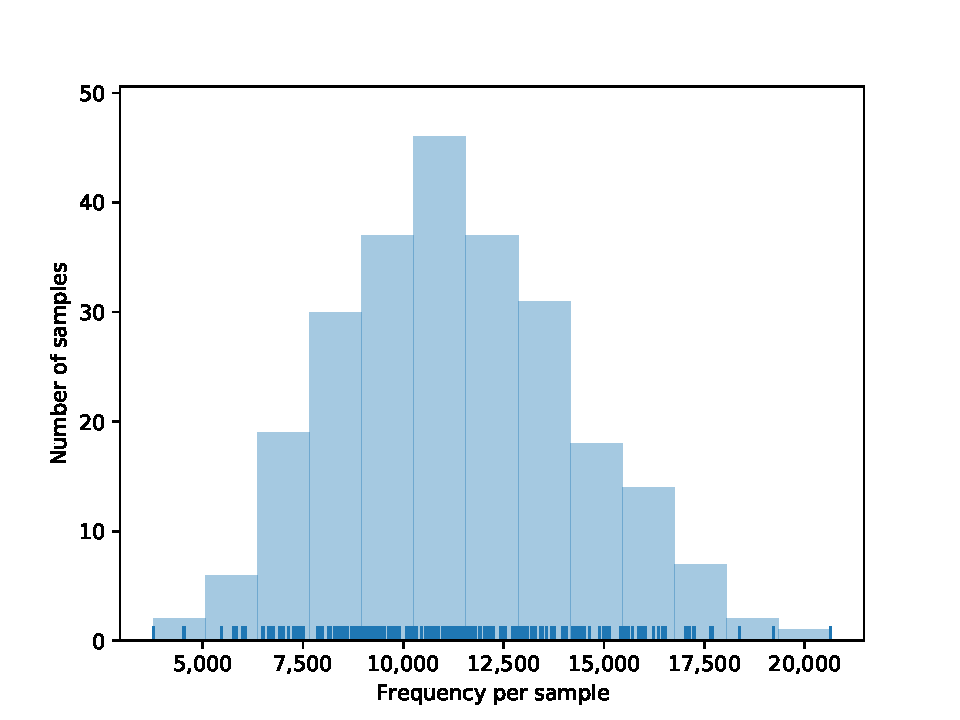
\includegraphics[width=0.6 \linewidth]{figures/Rarefaction/DADA.pdf}
                \caption{Frequency and Number per Sample by DADA2}
                \label{fig:frequency-sample-dada2}
            \end{figure}

            \begin{figure}[p]
                \centering
                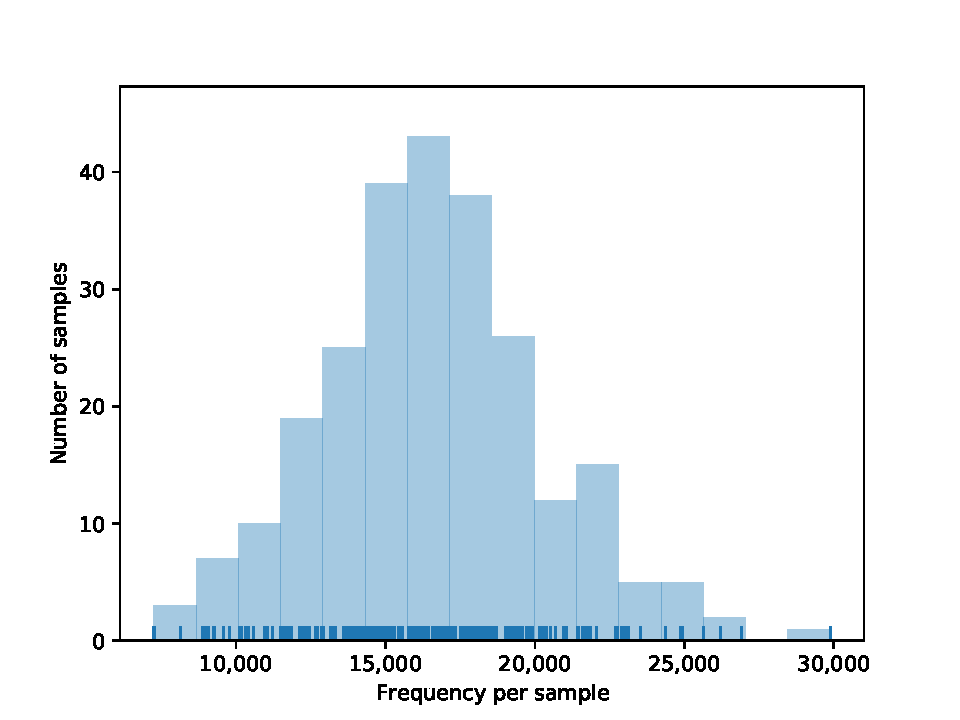
\includegraphics[width=0.6 \linewidth]{figures/Rarefaction/Deblur.pdf}
                \caption{Frequency and Number per Sample by Deblur}
                \label{fig:frequency-sample-deblur}
            \end{figure}

        \subsection{Alpha-diversity}
            Alpha-diversity analysis with DADA2 was done: Evenness index (Table \ref{tb:alpha-evenness-dada2} and Figure \ref{fig:evenness-dada2}), Faith PD (Table \ref{tb:alpha-faith-dada2} and Figure \ref{fig:faith-dada2}), observed feature index (Table \ref{tb:alpha-observed-dada2} and Figure \ref{fig:observed-dada2}) and Shannon's diversity index (Table \ref{tb:alpha-shannon-dada2} and Figure \ref{fig:shannon-dada2}). Also, alpha-diversity analysis with DADA2 was done: Evenness index (Table \ref{tb:alpha-evenness-deblur} and Figure \ref{fig:evenness-deblur}), Faith PD (Table \ref{tb:alpha-faith-deblur} and Figure \ref{fig:faith-deblur}), observed feature index (Table \ref{tb:alpha-observed-deblur} and Figure \ref{fig:observed-deblur}) and Shannon's diversity index (Table \ref{tb:alpha-shannon-deblur} and Figure \ref{fig:shannon-deblur}). Moreover, Kruskal-Wallis tests among all groups are shown as table \ref{tb:alpha-all-dada2} (with DADA2) and table \ref{tb:alpha-all-deblur} (with Deblur).

            \begin{table}[p]
                \centering
                \caption{Kruskal-Wallis Tests among All Group with DADA2}
                \label{tb:alpha-all-dada2}
                \csvautobooktabular{csv/AlphaDiversity/DADA2/all.csv}
            \end{table}

            \begin{table}[p]
                \centering
                \caption{Kruskal-Wallis Tests from Evenness Index with DADA2}
                \label{tb:alpha-evenness-dada2}
                \csvautobooktabular{csv/AlphaDiversity/DADA2/evenness.csv}
            \end{table}

            \begin{table}[p]
                \centering
                \caption{Kruskal-Wallis Tests from Faith PD Index with DADA2}
                \label{tb:alpha-faith-dada2}
                \csvautobooktabular{csv/AlphaDiversity/DADA2/faith.csv}
            \end{table}

            \begin{table}[p]
                \centering
                \caption{Kruskal-Wallis Tests from Observed Features Index with DADA2}
                \label{tb:alpha-observed-dada2}
                \csvautobooktabular{csv/AlphaDiversity/DADA2/observed.csv}
            \end{table}

            \begin{table}[p]
                \centering
                \caption{Kruskal-Wallis Tests from Shannon's Diversity Index with DADA2}
                \label{tb:alpha-shannon-dada2}
                \csvautobooktabular{csv/AlphaDiversity/DADA2/shannon.csv}
            \end{table}

            \begin{figure}[p]
                \centering
                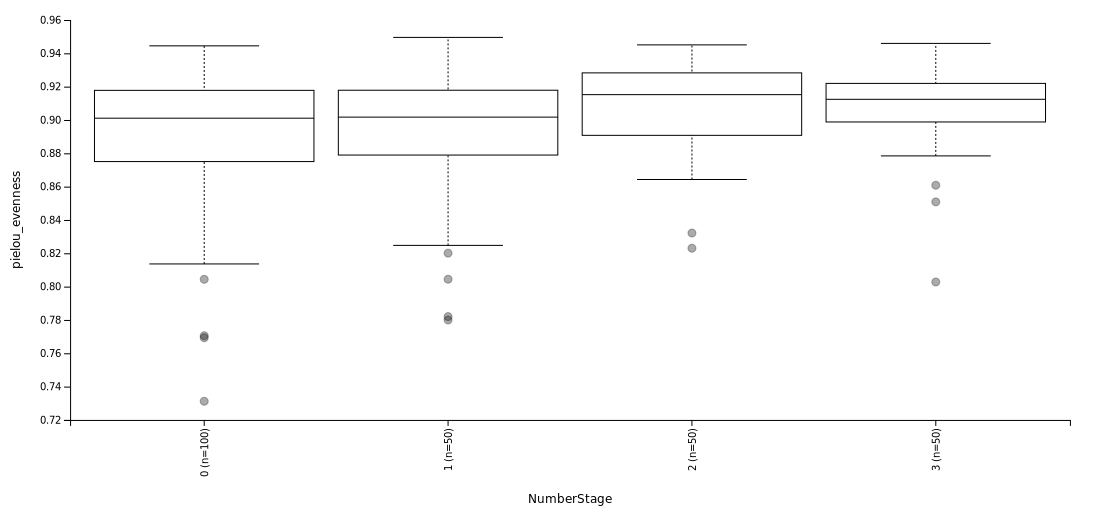
\includegraphics[width=0.8 \linewidth]{figures/AlphaDiversity/DADA2/evenness.png}
                \caption{Evenness Index from DADA2}
                \label{fig:evenness-dada2}
            \end{figure}

            \begin{figure}[p]
                \centering
                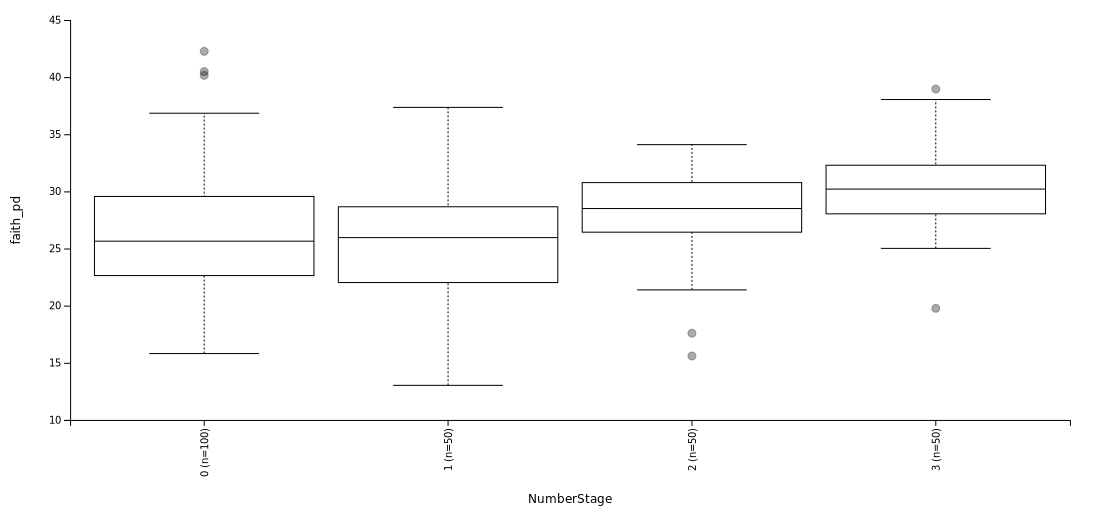
\includegraphics[width=0.8 \linewidth]{figures/AlphaDiversity/DADA2/faith.png}
                \caption{Faith PD Index from DADA2}
                \label{fig:faith-dada2}
            \end{figure}

            \begin{figure}[p]
                \centering
                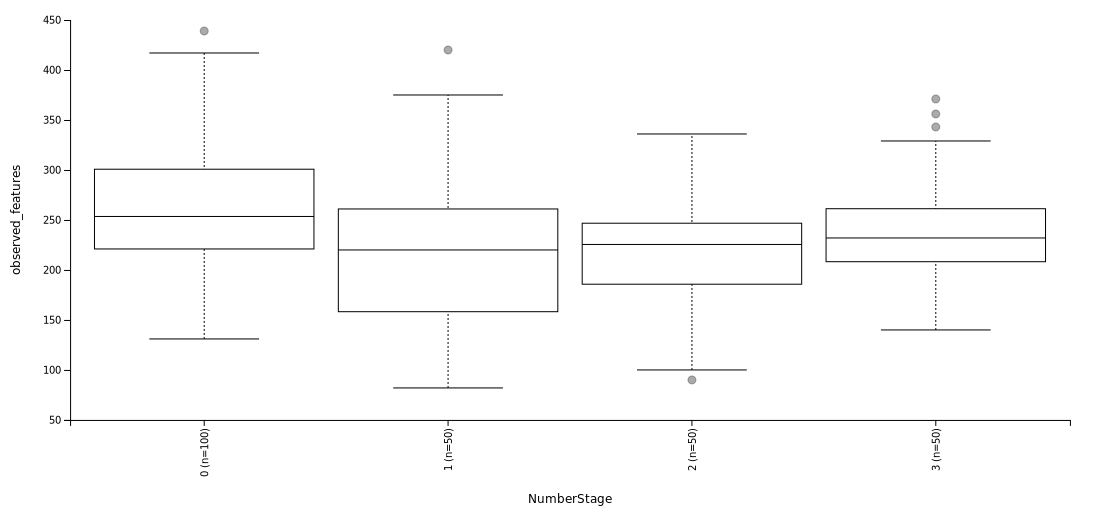
\includegraphics[width=0.8 \linewidth]{figures/AlphaDiversity/DADA2/observed.png}
                \caption{Observed Features Index from DADA2}
                \label{fig:observed-dada2}
            \end{figure}

            \begin{figure}[p]
                \centering
                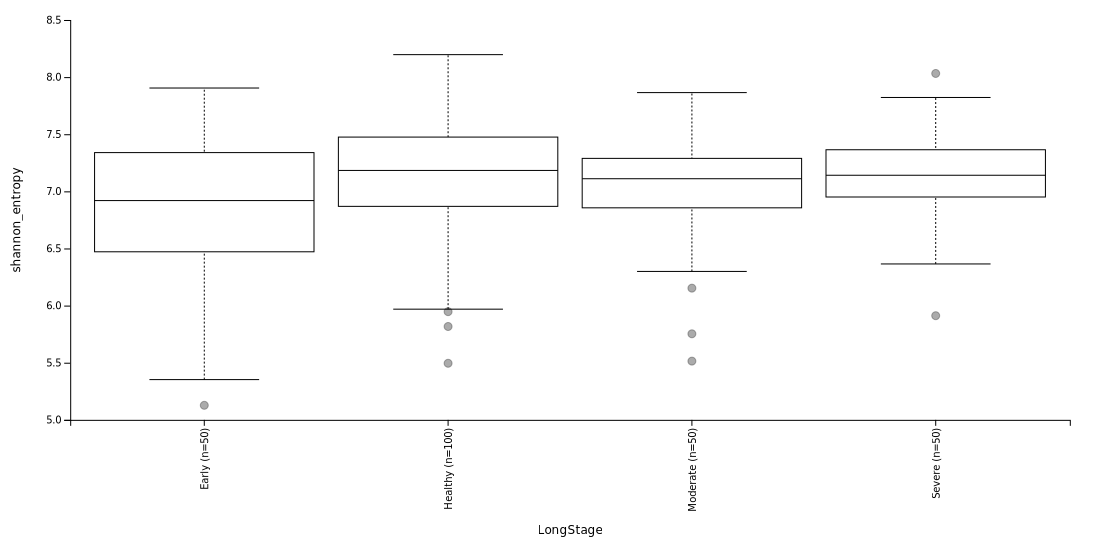
\includegraphics[width=0.8 \linewidth]{figures/AlphaDiversity/DADA2/shannon.png}
                \caption{Shannon's Diversity Index from DADA2}
                \label{fig:shannon-dada2}
            \end{figure}

            \begin{table}[p]
                \centering
                \caption{Kruskal-Wallis Tests among All Group with Deblur}
                \label{tb:alpha-all-deblur}
                \csvautobooktabular{csv/AlphaDiversity/Deblur/all.csv}
            \end{table}

            \begin{table}[p]
                \centering
                \caption{Kruskal-Wallis Tests from Evenness Index with Deblur}
                \label{tb:alpha-evenness-deblur}
                \csvautobooktabular{csv/AlphaDiversity/Deblur/evenness.csv}
            \end{table}

            \begin{table}[p]
                \centering
                \caption{Kruskal-Wallis Tests from Faith PD Index with Deblur}
                \label{tb:alpha-faith-deblur}
                \csvautobooktabular{csv/AlphaDiversity/Deblur/faith.csv}
            \end{table}

            \begin{table}[p]
                \centering
                \caption{Kruskal-Wallis Tests from Observed Features Index with Deblur}
                \label{tb:alpha-observed-deblur}
                \csvautobooktabular{csv/AlphaDiversity/Deblur/observed.csv}
            \end{table}

            \begin{table}[p]
                \centering
                \caption{Kruskal-Wallis Tests from Shannon's Diversity Index with Deblur}
                \label{tb:alpha-shannon-deblur}
                \csvautobooktabular{csv/AlphaDiversity/Deblur/shannon.csv}
            \end{table}

            \begin{figure}[p]
                \centering
                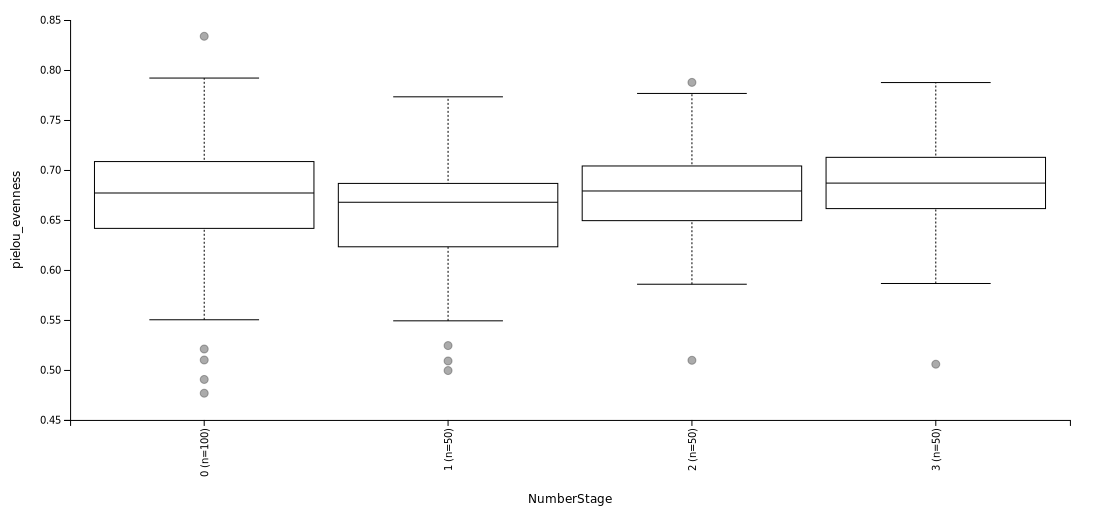
\includegraphics[width=0.8 \linewidth]{figures/AlphaDiversity/Deblur/evenness.png}
                \caption{Evenness Index from Deblur}
                \label{fig:evenness-deblur}
            \end{figure}

            \begin{figure}[p]
                \centering
                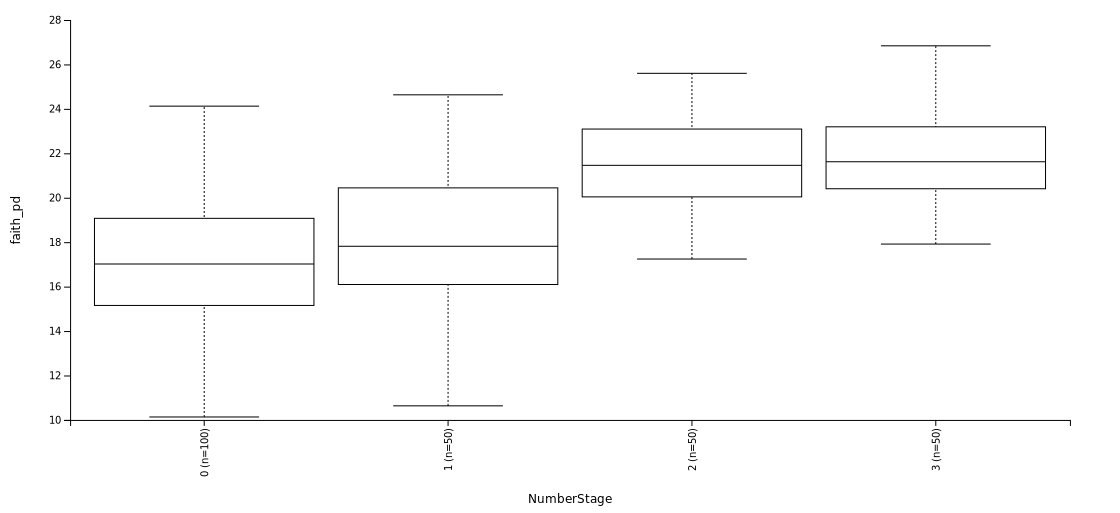
\includegraphics[width=0.8 \linewidth]{figures/AlphaDiversity/Deblur/faith.png}
                \caption{Faith PD Index from Deblur}
                \label{fig:faith-deblur}
            \end{figure}

            \begin{figure}[p]
                \centering
                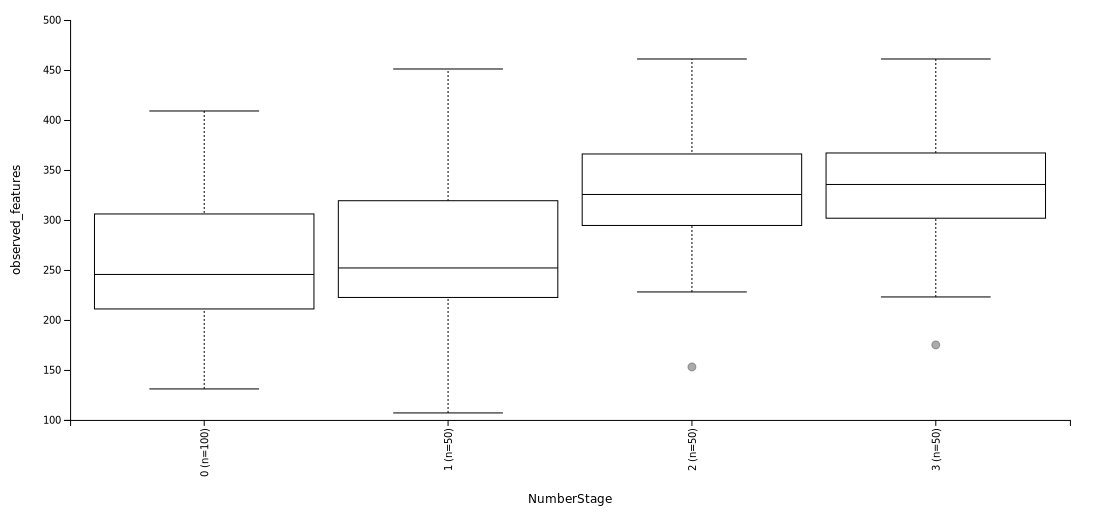
\includegraphics[width=0.8 \linewidth]{figures/AlphaDiversity/Deblur/observed.png}
                \caption{Observed Features Index from Deblur}
                \label{fig:observed-deblur}
            \end{figure}

            \begin{figure}[p]
                \centering
                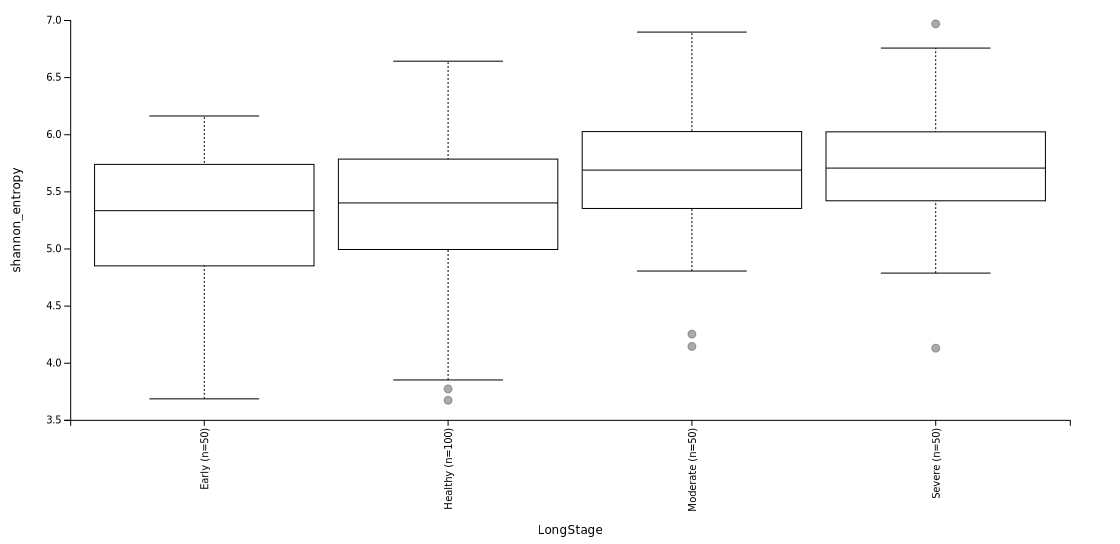
\includegraphics[width=0.8 \linewidth]{figures/AlphaDiversity/Deblur/shannon.png}
                \caption{Shannon's Diversity Index from Deblur}
                \label{fig:shannon-deblur}
            \end{figure}

        \subsection{Beta-diversity}
            Beta-diversity analysis with DADA2 was done: Bray-Curtis distance (Table \ref{tb:bray-dada2} and Figure \ref{fig:bray-dada2}), Jaccard distance (Table \ref{tb:jaccard-dada2} and Figure \ref{fig:jaccard-dada2}), unweighted UniFrac distance (Table \ref{tb:unweighted-dada2} and Figure \ref{fig:unweighted-dada2}) and weighted UniFrac distance (Table \ref{tb:weighted-dada2} and Figure \ref{fig:unweighted-dada2}). Also, beta-diversity analysis with Deblur was done: Bray-Curtis distance (Table \ref{tb:bray-deblur} and Figure \ref{fig:bray-deblur}), Jaccard distance (Table \ref{tb:jaccard-deblur} and Figure \ref{fig:jaccard-deblur}), unweighted UniFrac distance (Table \ref{tb:unweighted-deblur} and Figure \ref{fig:unweighted-deblur}) and weighted UniFrac distance (Table \ref{tb:weighted-deblur} and Figure \ref{fig:unweighted-deblur}).

            \begin{table}[p]
                \centering
                \caption{Bray-Curtis Distance Index with DADA2}
                \label{tb:bray-dada2}
                \csvautobooktabular{csv/BetaDiversity/DADA2/Bray.csv}
            \end{table}

            \begin{table}[p]
                \centering
                \caption{Jaccard Distance Index with DADA2}
                \label{tb:jaccard-dada2}
                \csvautobooktabular{csv/BetaDiversity/DADA2/Jaccard.csv}
            \end{table}

            \begin{table}[p]
                \centering
                \caption{Unweighted UniFrac Distance Index with DADA2}
                \label{tb:unweighted-dada2}
                \csvautobooktabular{csv/BetaDiversity/DADA2/UnweightedUniFrac.csv}
            \end{table}

            \begin{table}[p]
                \centering
                \caption{Weighted UniFrac Distance Index with DADA2}
                \label{tb:weighted-dada2}
                \csvautobooktabular{csv/BetaDiversity/DADA2/WeightedUniFrac.csv}
            \end{table}

            \begin{figure}[p]
                \centering
                $\begin{array}{cc}
                    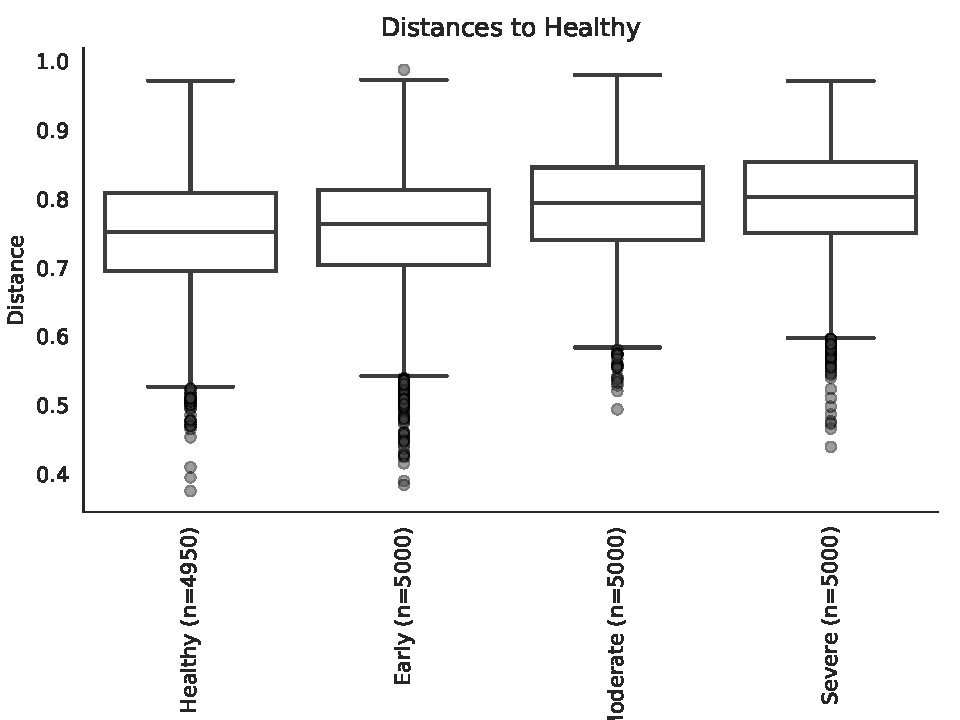
\includegraphics[width=0.4 \linewidth]{figures/BetaDiversity/DADA2/Bray/Healthy.pdf}
                    &
                    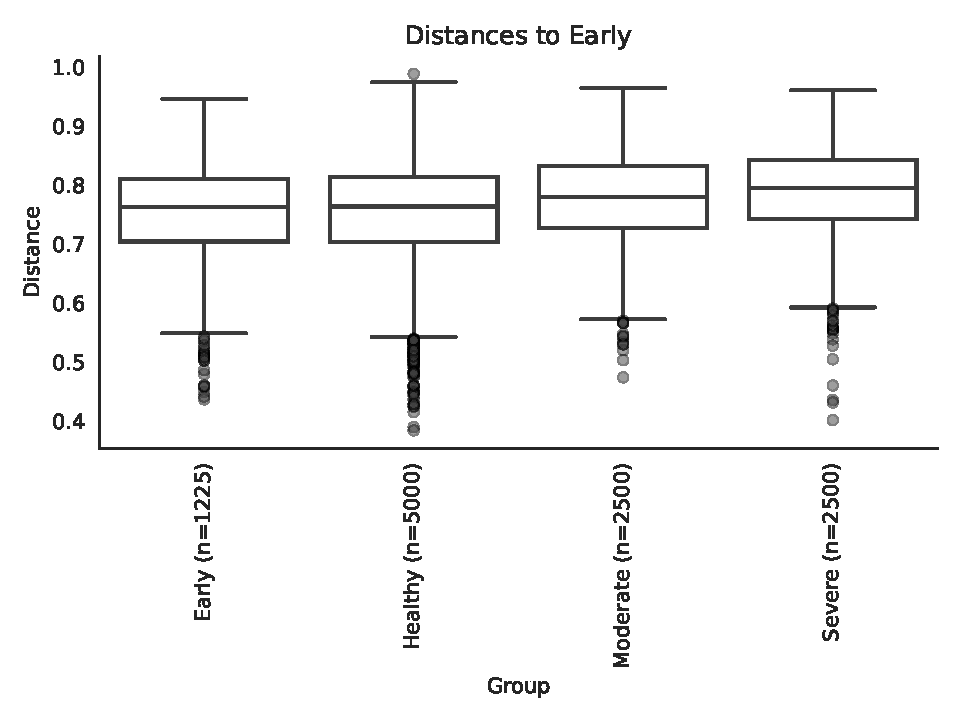
\includegraphics[width=0.4 \linewidth]{figures/BetaDiversity/DADA2/Bray/Early.pdf}
                    \\
                    \mbox{(a) Healthy} & \mbox{(b) Early} \\

                    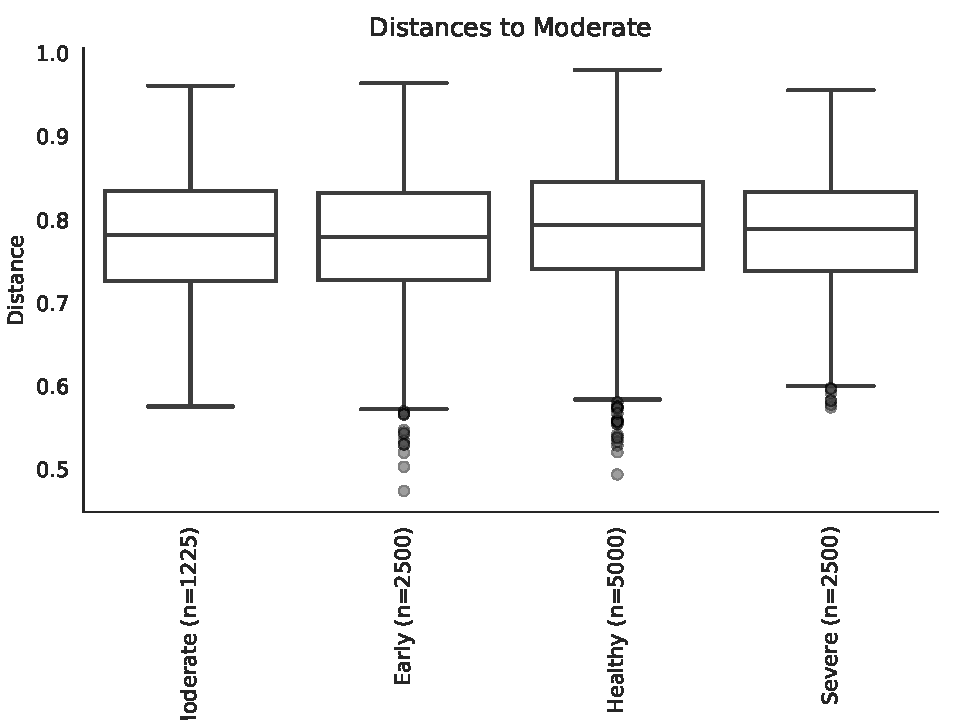
\includegraphics[width=0.4 \linewidth]{figures/BetaDiversity/DADA2/Bray/Moderate.pdf}
                    &
                    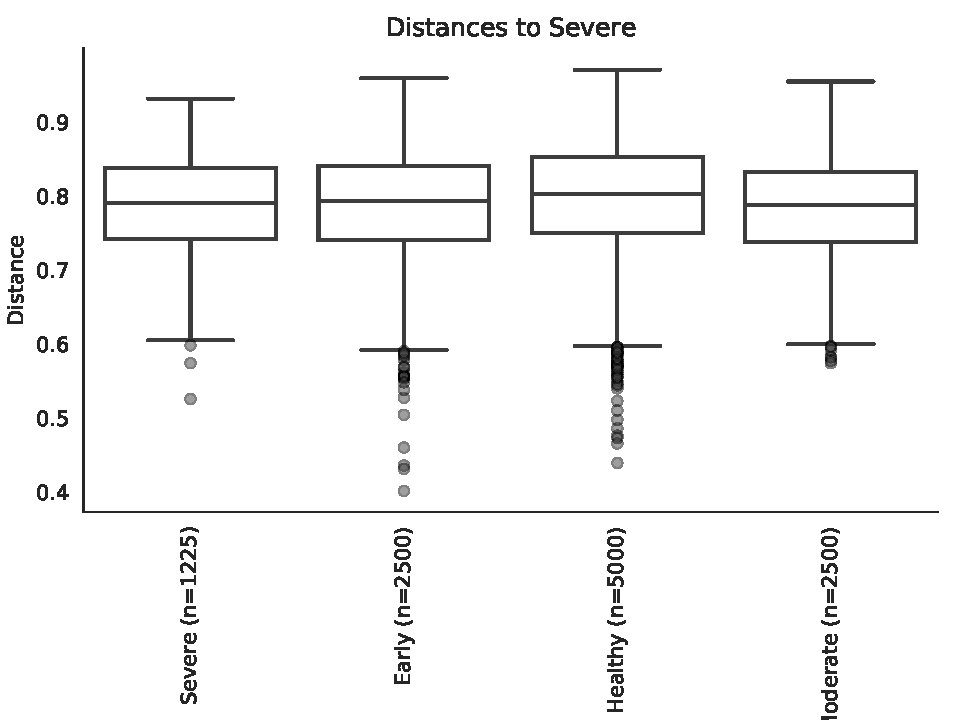
\includegraphics[width=0.4 \linewidth]{figures/BetaDiversity/DADA2/Bray/Severe.pdf}
                    \\
                    \mbox{(c) Moderate} & \mbox{(d) Severe} \\
                \end{array}$
                \caption{Bray-Curtis Distance Index with DADA2}
                \label{fig:bray-dada2}
            \end{figure}

            \begin{figure}[p]
                \centering
                $\begin{array}{cc}
                    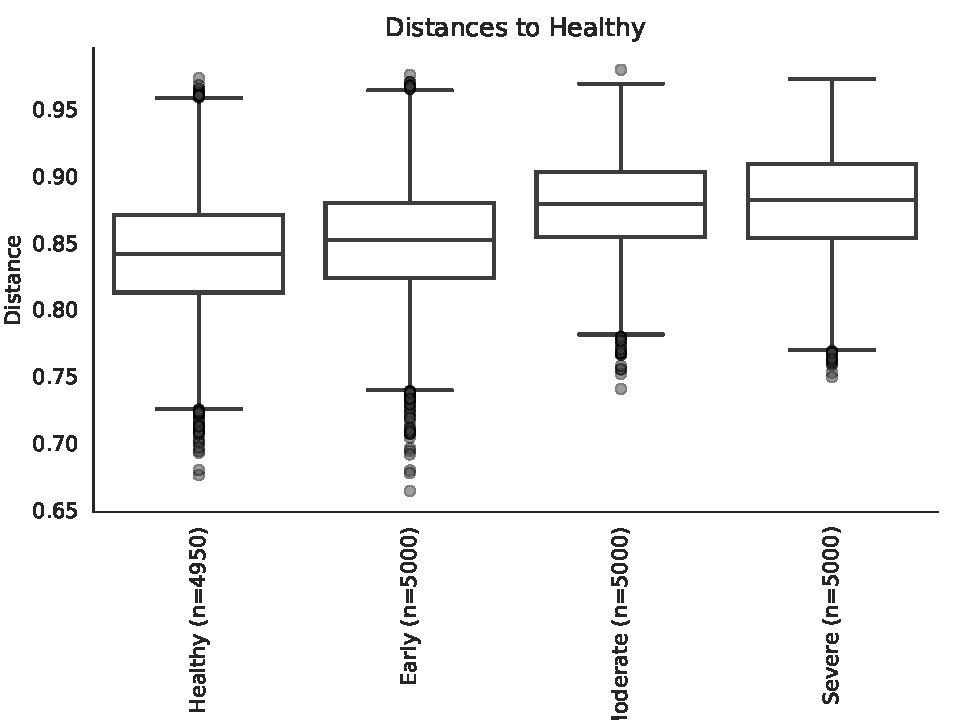
\includegraphics[width=0.4 \linewidth]{figures/BetaDiversity/DADA2/Jaccard/Healthy.pdf}
                    &
                    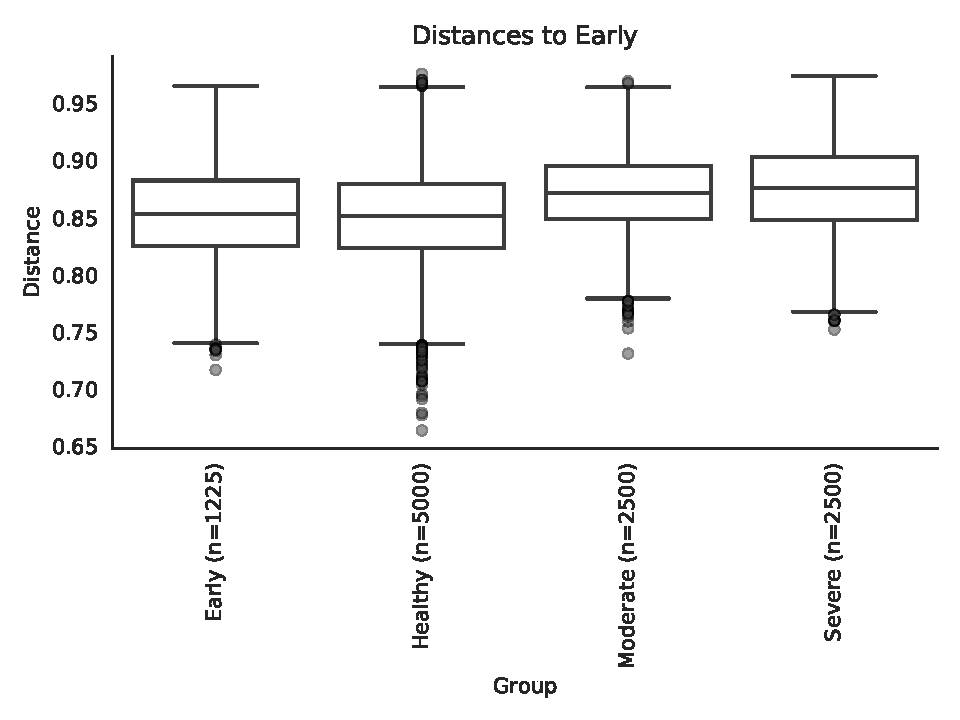
\includegraphics[width=0.4 \linewidth]{figures/BetaDiversity/DADA2/Jaccard/Early.pdf}
                    \\
                    \mbox{(a) Healthy} & \mbox{(b) Early} \\

                    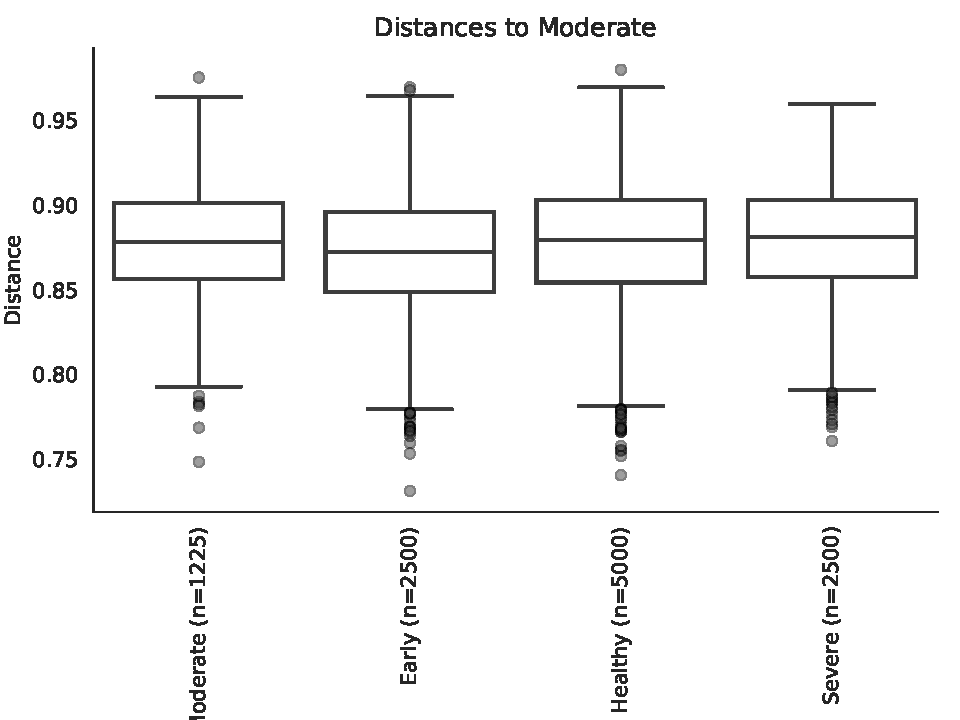
\includegraphics[width=0.4 \linewidth]{figures/BetaDiversity/DADA2/Jaccard/Moderate.pdf}
                    &
                    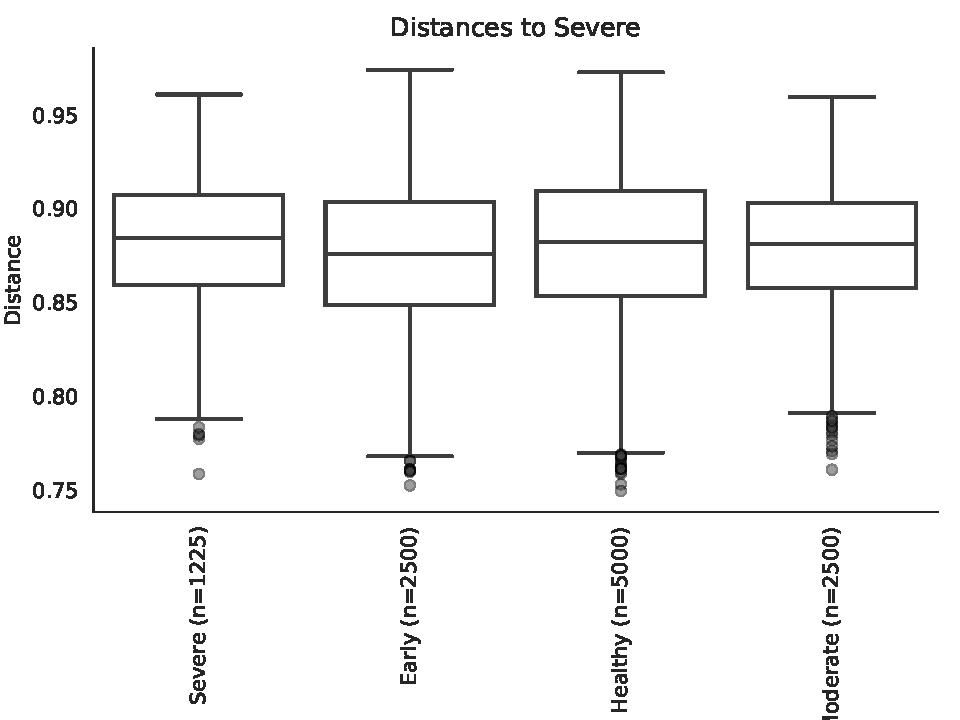
\includegraphics[width=0.4 \linewidth]{figures/BetaDiversity/DADA2/Jaccard/Severe.pdf}
                    \\
                    \mbox{(c) Moderate} & \mbox{(d) Severe} \\
                \end{array}$
                \caption{Jaccard Distance Index with DADA2}
                \label{fig:jaccard-dada2}
            \end{figure}

            \begin{figure}[p]
                \centering
                $\begin{array}{cc}
                    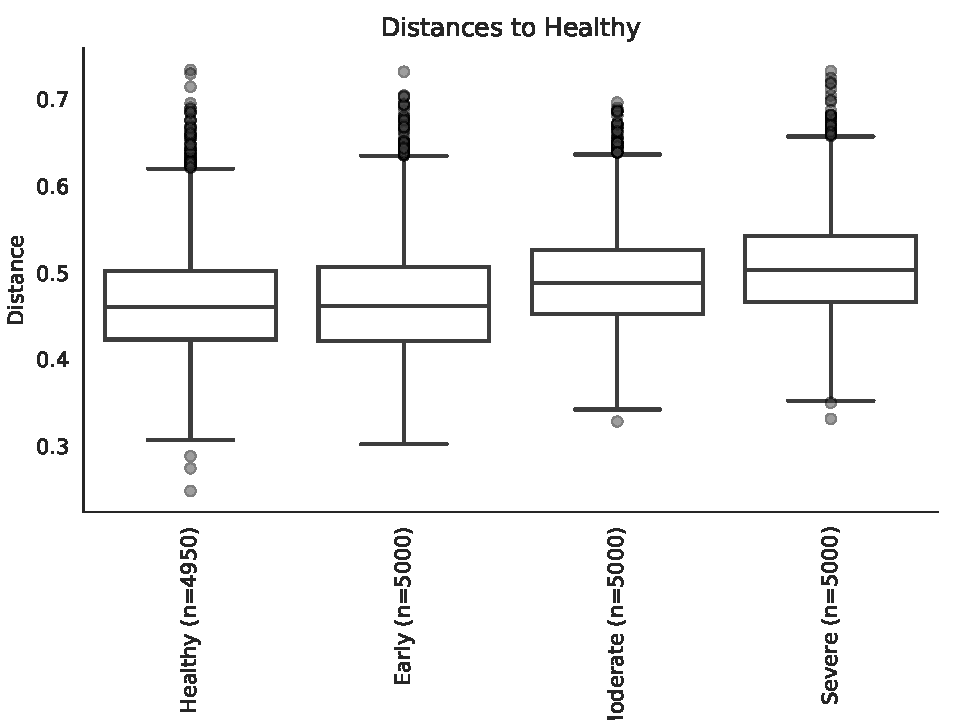
\includegraphics[width=0.4 \linewidth]{figures/BetaDiversity/DADA2/UnweightedUnifrac/Healthy.pdf}
                    &
                    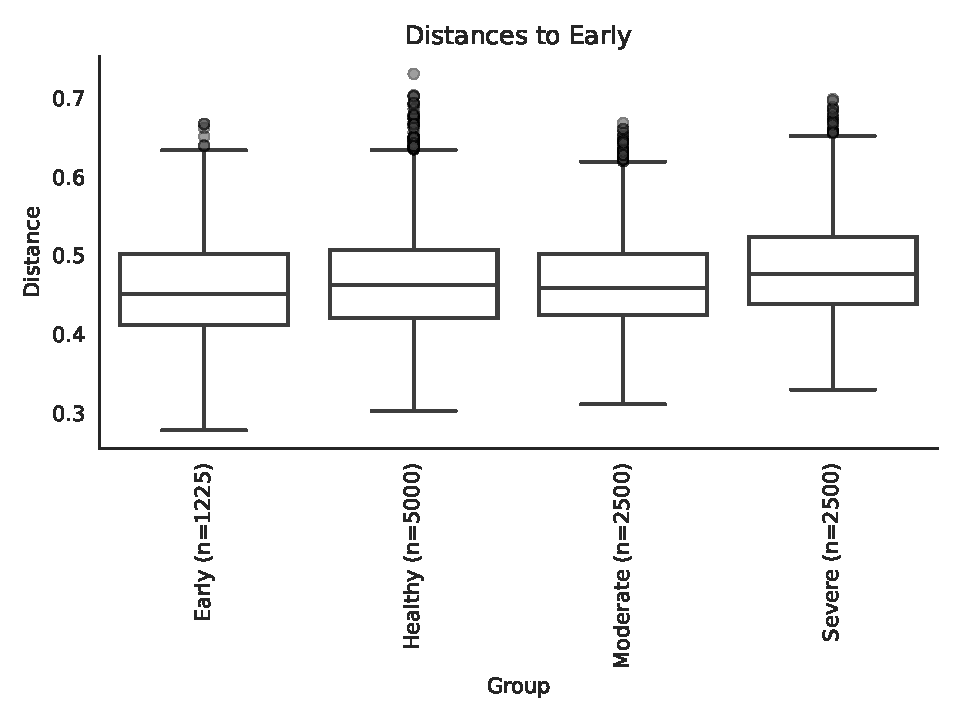
\includegraphics[width=0.4 \linewidth]{figures/BetaDiversity/DADA2/UnweightedUnifrac/Early.pdf}
                    \\
                    \mbox{(a) Healthy} & \mbox{(b) Early} \\

                    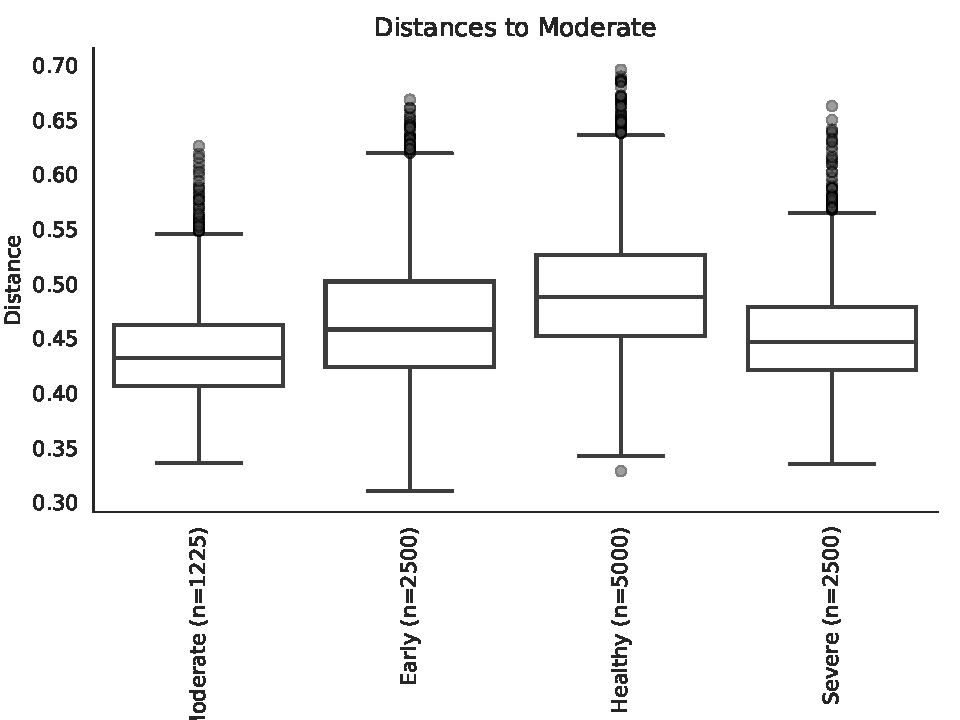
\includegraphics[width=0.4 \linewidth]{figures/BetaDiversity/DADA2/UnweightedUnifrac/Moderate.pdf}
                    &
                    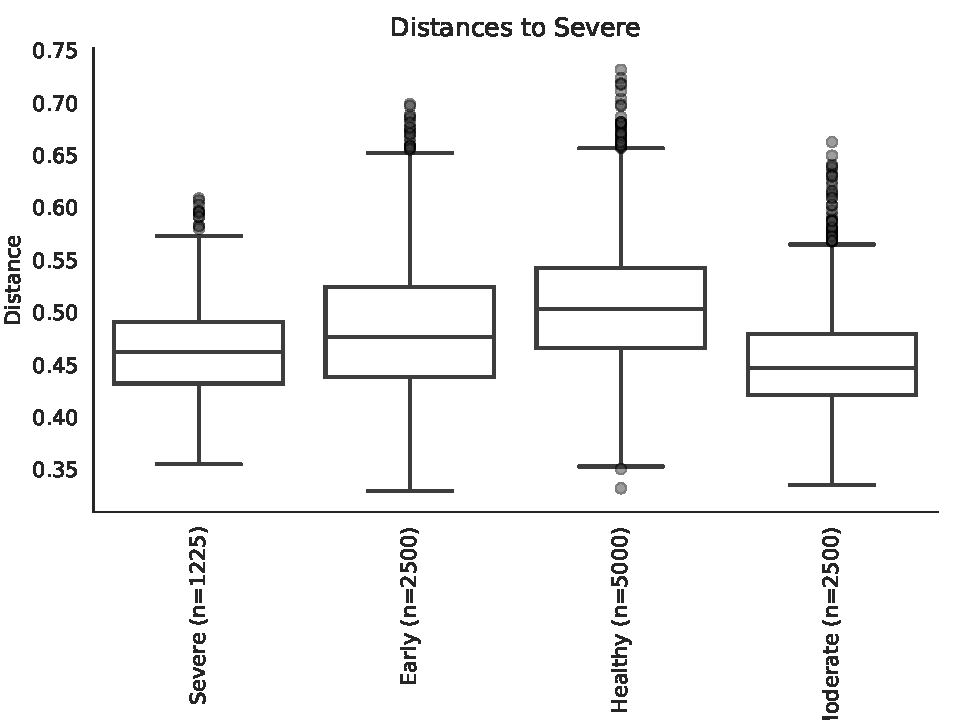
\includegraphics[width=0.4 \linewidth]{figures/BetaDiversity/DADA2/UnweightedUnifrac/Severe.pdf}
                    \\
                    \mbox{(c) Moderate} & \mbox{(d) Severe} \\
                \end{array}$
                \caption{Unweighted Unifrac Distance Index with DADA2}
                \label{fig:unweighted-dada2}
            \end{figure}

            \begin{figure}[p]
                \centering
                $\begin{array}{cc}
                    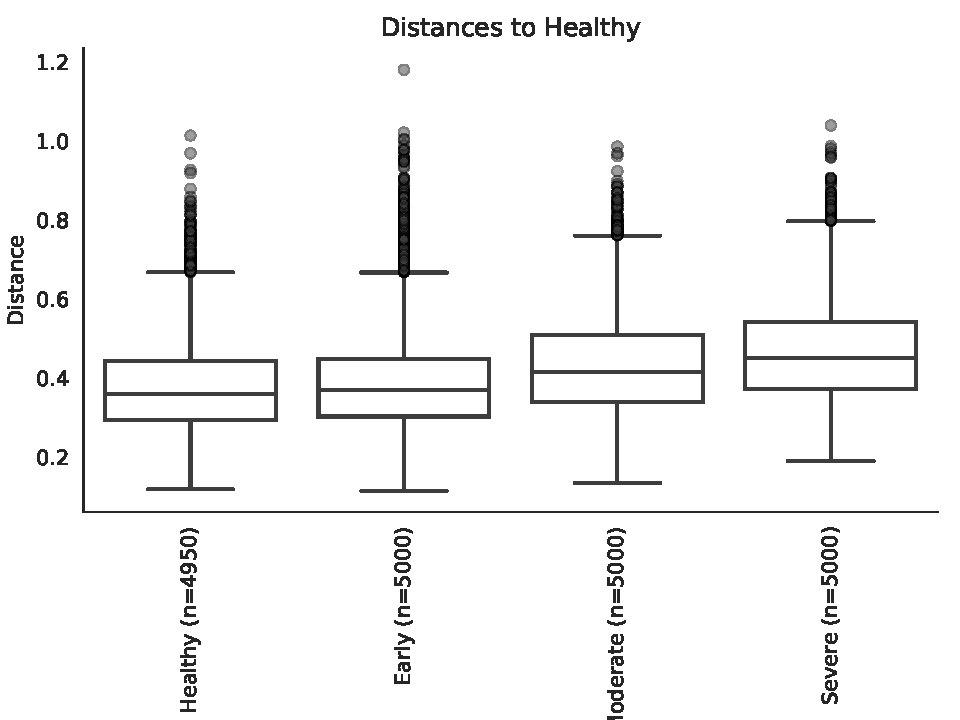
\includegraphics[width=0.4 \linewidth]{figures/BetaDiversity/DADA2/WeightedUnifrac/Healthy.pdf}
                    &
                    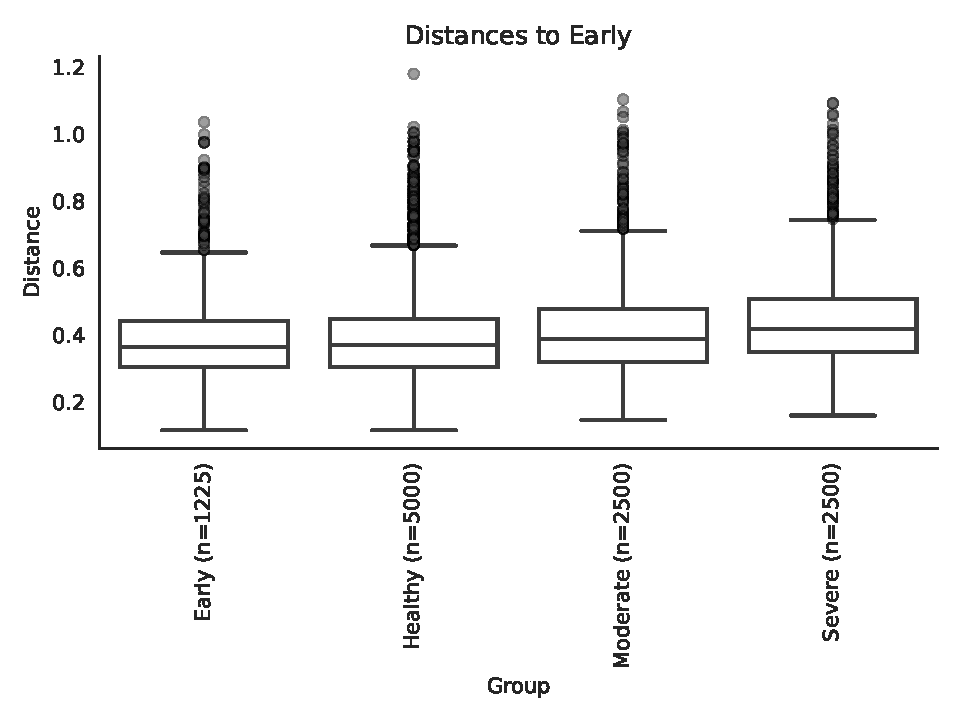
\includegraphics[width=0.4 \linewidth]{figures/BetaDiversity/DADA2/WeightedUnifrac/Early.pdf}
                    \\
                    \mbox{(a) Healthy} & \mbox{(b) Early} \\

                    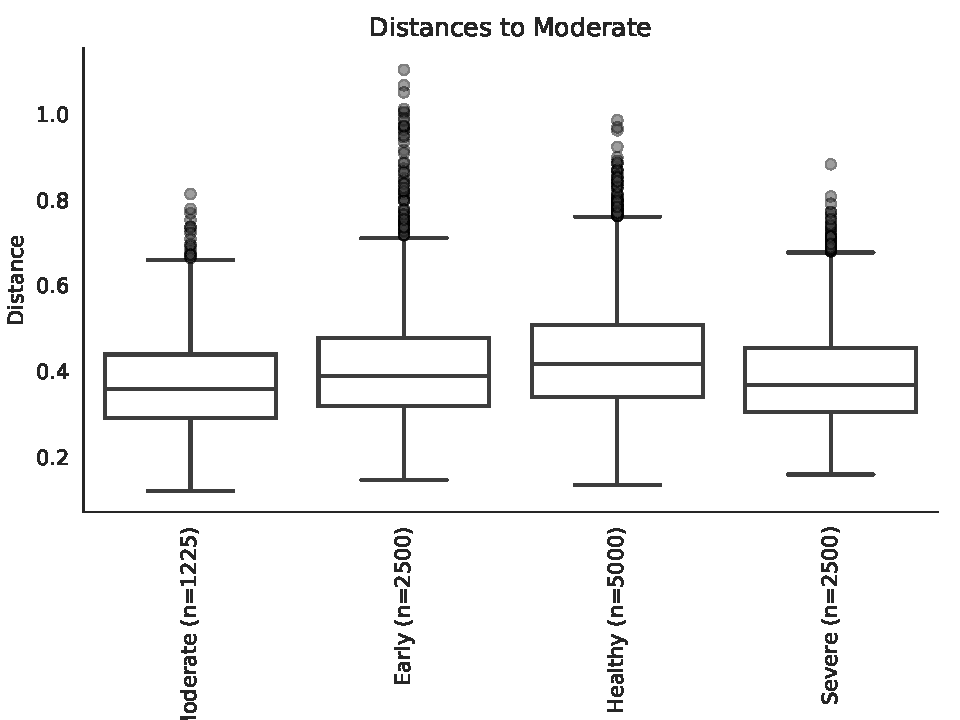
\includegraphics[width=0.4 \linewidth]{figures/BetaDiversity/DADA2/WeightedUnifrac/Moderate.pdf}
                    &
                    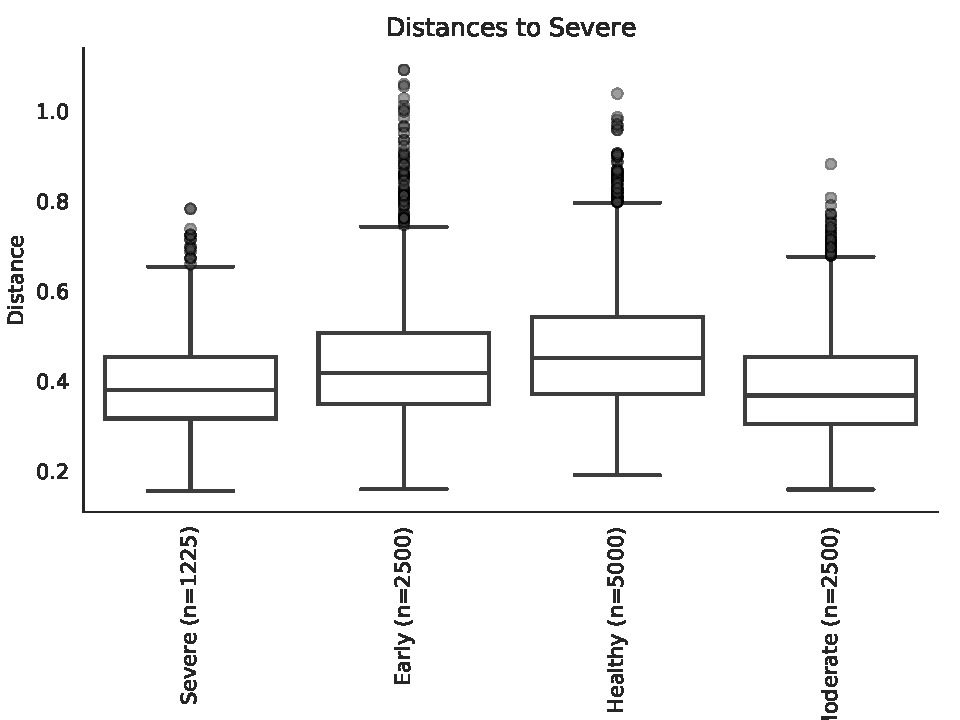
\includegraphics[width=0.4 \linewidth]{figures/BetaDiversity/DADA2/WeightedUnifrac/Severe.pdf}
                    \\
                    \mbox{(c) Moderate} & \mbox{(d) Severe} \\
                \end{array}$
                \caption{Weighted Unifrac Distance Index with DADA2}
                \label{fig:weighted-dada2}
            \end{figure}

            \begin{table}[p]
                \centering
                \caption{Bray-Curtis Distance Index with Deblur}
                \label{tb:bray-deblur}
                \csvautobooktabular{csv/BetaDiversity/Deblur/Bray.csv}
            \end{table}

            \begin{table}[p]
                \centering
                \caption{Jaccard Distance Index with Deblur}
                \label{tb:jaccard-deblur}
                \csvautobooktabular{csv/BetaDiversity/Deblur/Jaccard.csv}
            \end{table}

            \begin{table}[p]
                \centering
                \caption{Unweighted UniFrac Distance Index with Deblur}
                \label{tb:unweighted-deblur}
                \csvautobooktabular{csv/BetaDiversity/Deblur/UnweightedUniFrac.csv}
            \end{table}

            \begin{table}[p]
                \centering
                \caption{Weighted UniFrac Distance Index with Deblur}
                \label{tb:weighted-deblur}
                \csvautobooktabular{csv/BetaDiversity/Deblur/WeightedUniFrac.csv}
            \end{table}

            \begin{figure}[p]
                \centering
                $\begin{array}{cc}
                    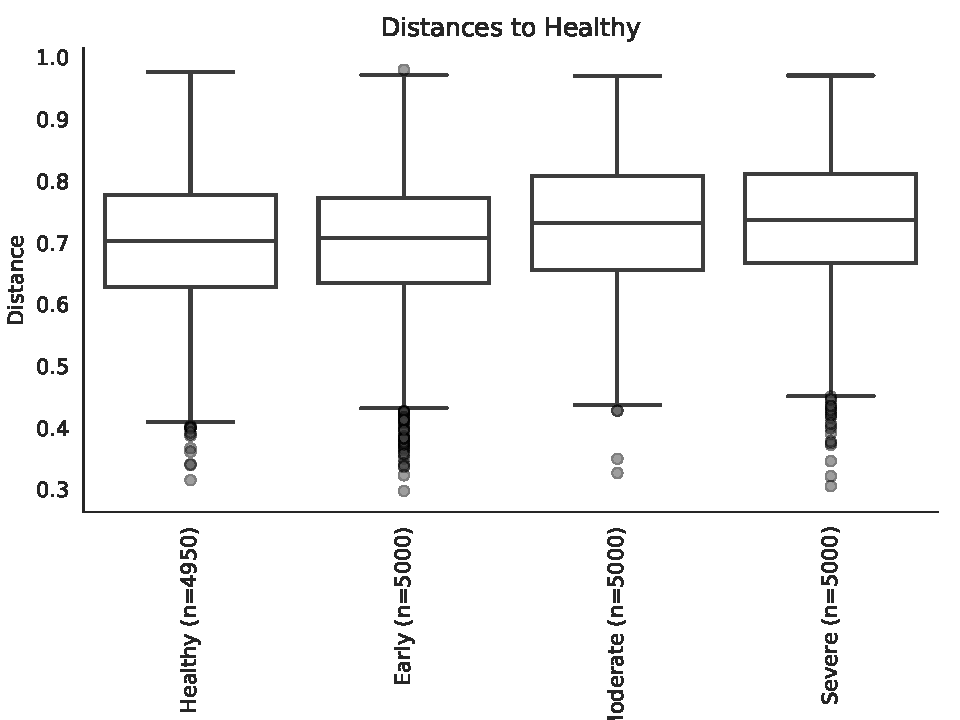
\includegraphics[width=0.4 \linewidth]{figures/BetaDiversity/Deblur/Bray/Healthy.pdf}
                    &
                    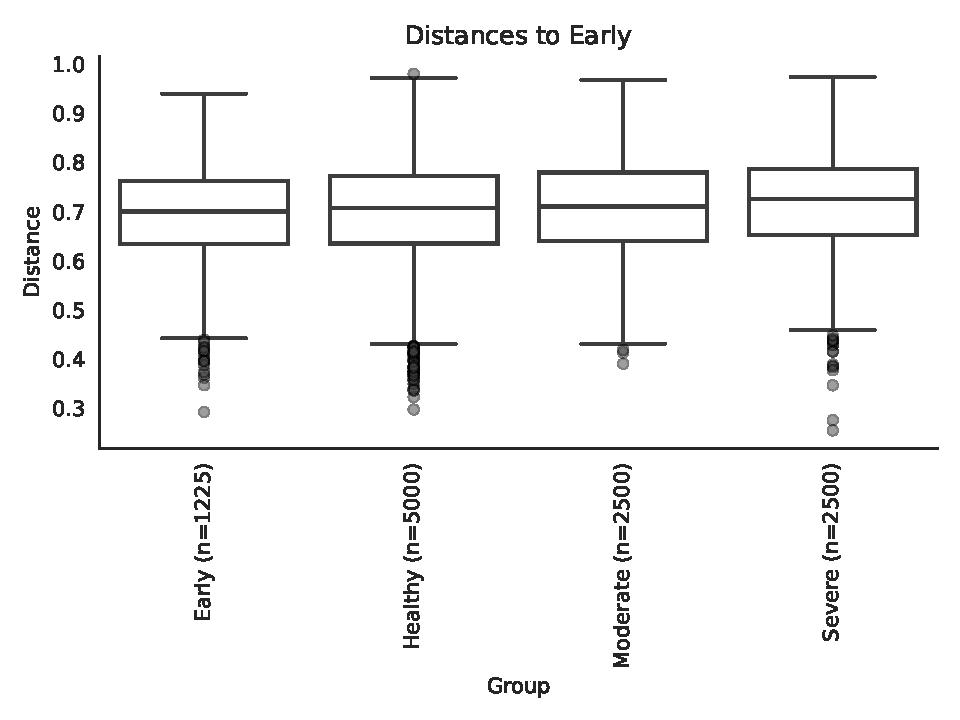
\includegraphics[width=0.4 \linewidth]{figures/BetaDiversity/Deblur/Bray/Early.pdf}
                    \\
                    \mbox{(a) Healthy} & \mbox{(b) Early} \\

                    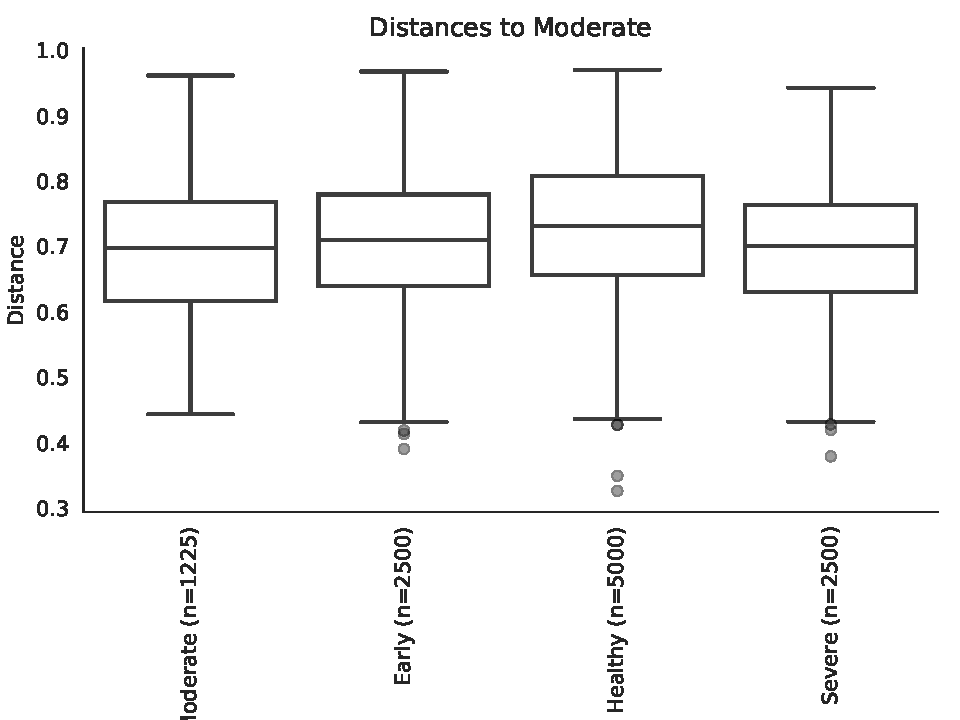
\includegraphics[width=0.4 \linewidth]{figures/BetaDiversity/Deblur/Bray/Moderate.pdf}
                    &
                    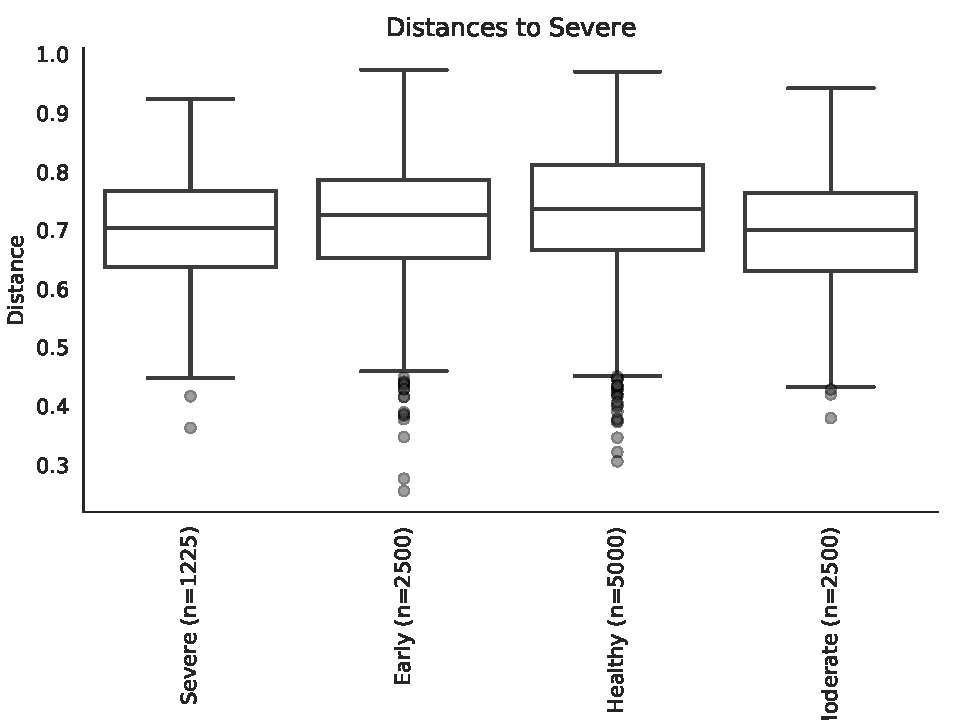
\includegraphics[width=0.4 \linewidth]{figures/BetaDiversity/Deblur/Bray/Severe.pdf}
                    \\
                    \mbox{(c) Moderate} & \mbox{(d) Severe} \\
                \end{array}$
                \caption{Bray-Curtis Distance Index with Deblur}
                \label{fig:bray-deblur}
            \end{figure}

            \begin{figure}[p]
                \centering
                $\begin{array}{cc}
                    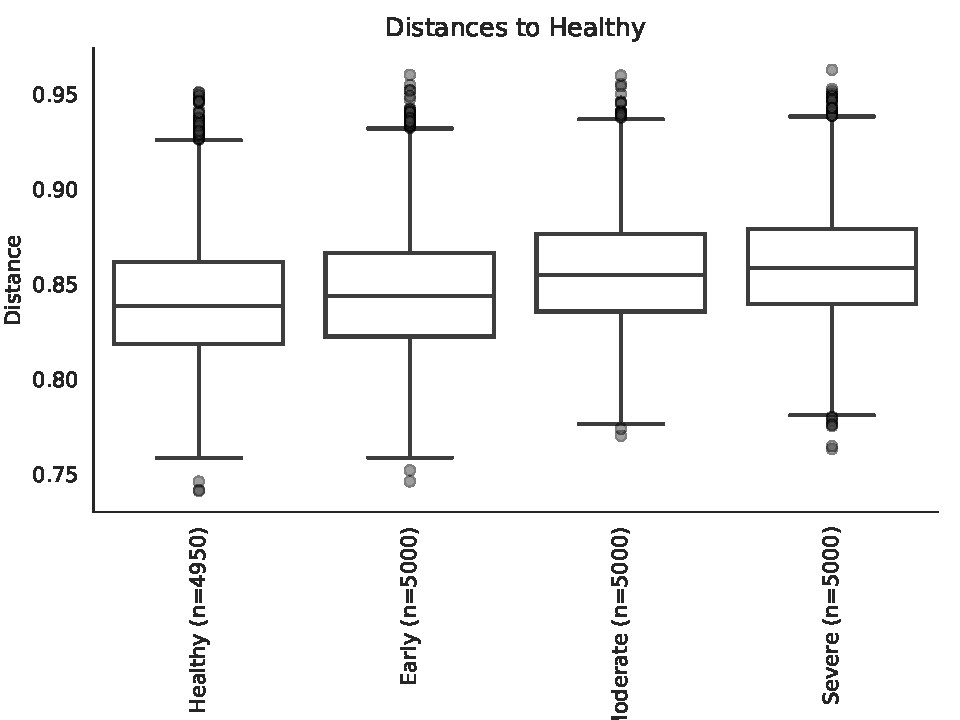
\includegraphics[width=0.4 \linewidth]{figures/BetaDiversity/Deblur/Jaccard/Healthy.pdf}
                    &
                    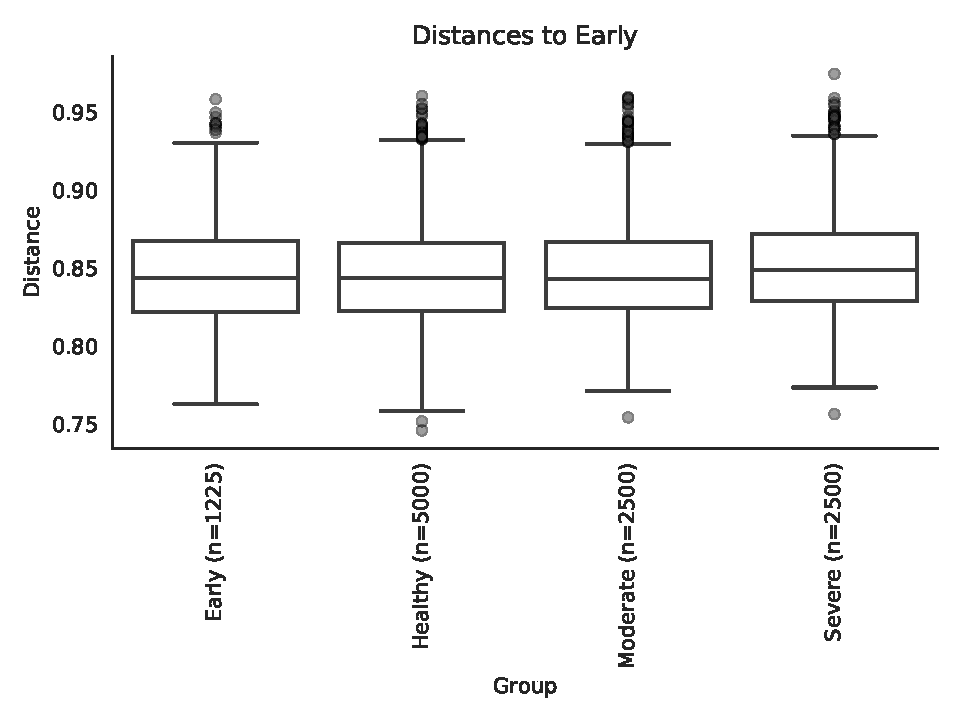
\includegraphics[width=0.4 \linewidth]{figures/BetaDiversity/Deblur/Jaccard/Early.pdf}
                    \\
                    \mbox{(a) Healthy} & \mbox{(b) Early} \\

                    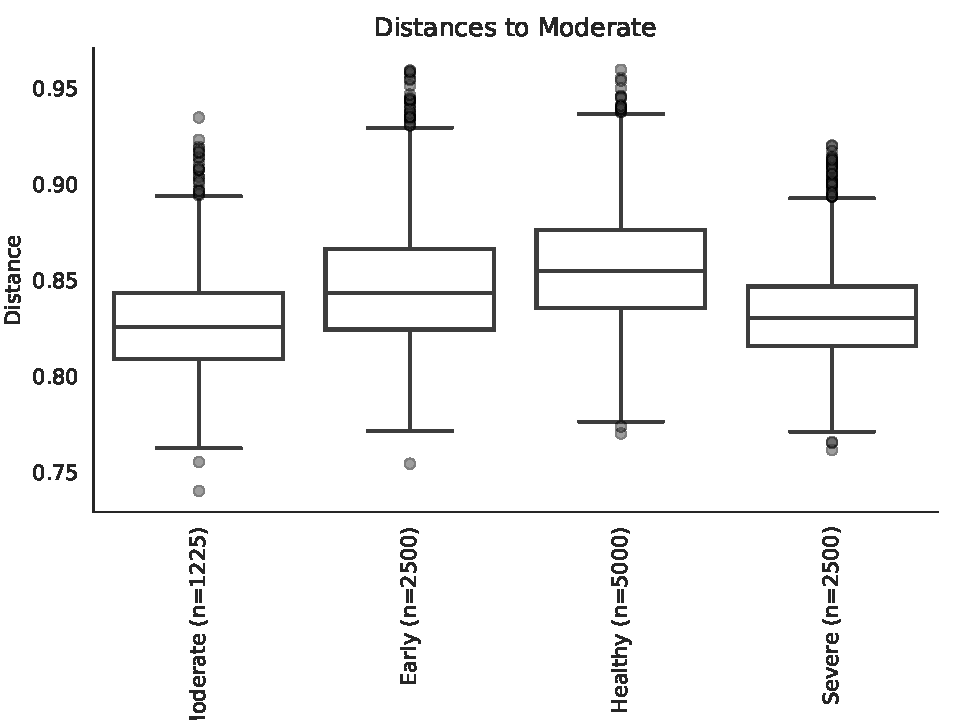
\includegraphics[width=0.4 \linewidth]{figures/BetaDiversity/Deblur/Jaccard/Moderate.pdf}
                    &
                    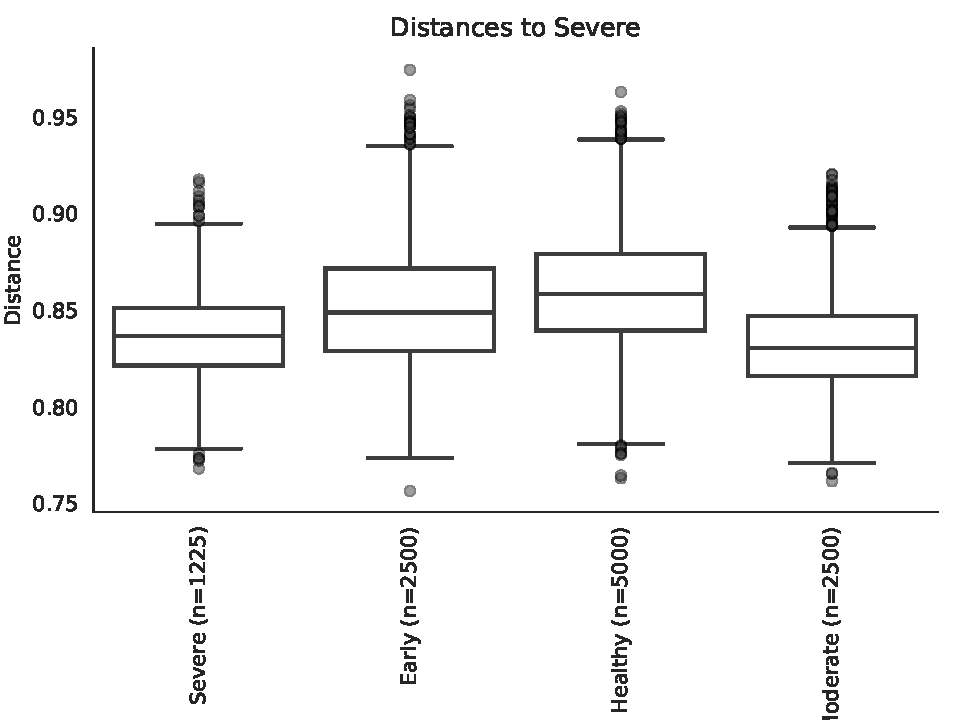
\includegraphics[width=0.4 \linewidth]{figures/BetaDiversity/Deblur/Jaccard/Severe.pdf}
                    \\
                    \mbox{(c) Moderate} & \mbox{(d) Severe} \\
                \end{array}$
                \caption{Jaccard Distance Index with Deblur}
                \label{fig:jaccard-deblur}
            \end{figure}

            \begin{figure}[p]
                \centering
                $\begin{array}{cc}
                    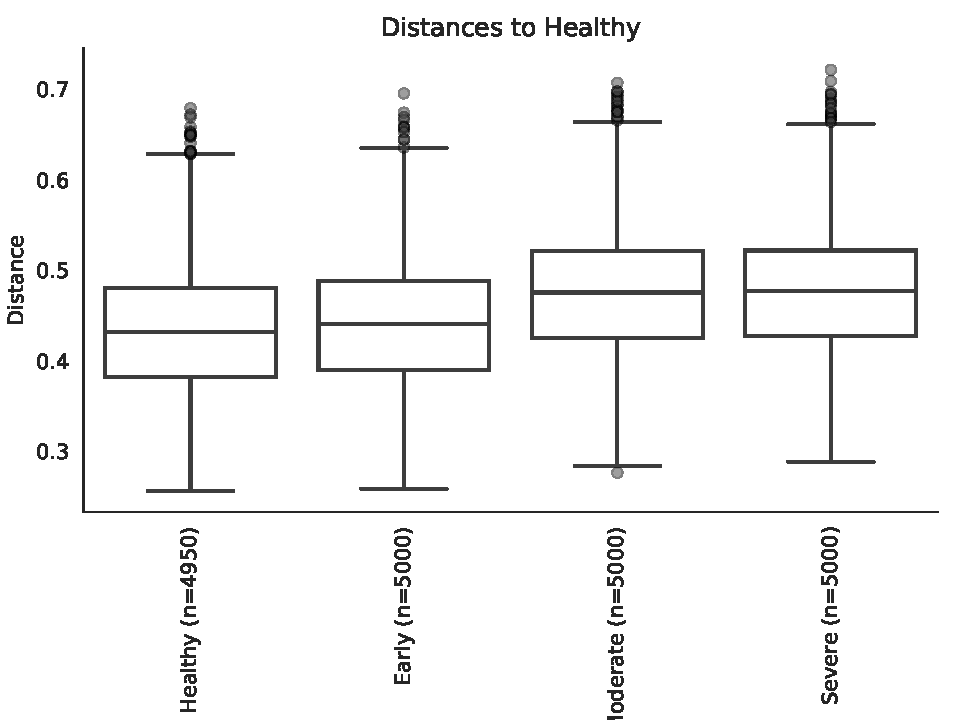
\includegraphics[width=0.4 \linewidth]{figures/BetaDiversity/Deblur/UnweightedUnifrac/Healthy.pdf}
                    &
                    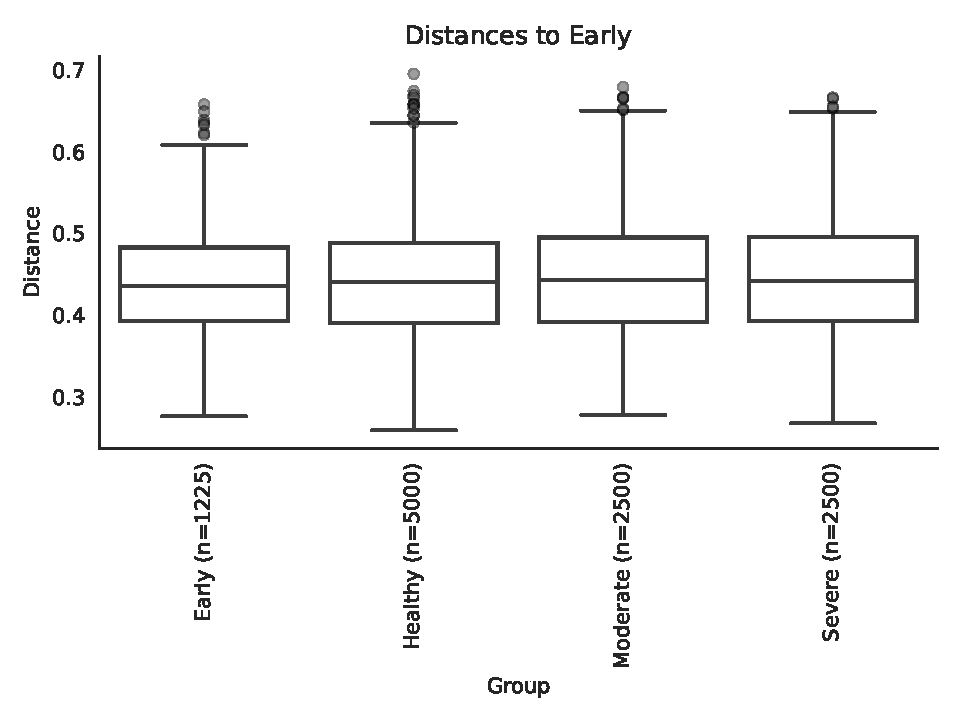
\includegraphics[width=0.4 \linewidth]{figures/BetaDiversity/Deblur/UnweightedUnifrac/Early.pdf}
                    \\
                    \mbox{(a) Healthy} & \mbox{(b) Early} \\

                    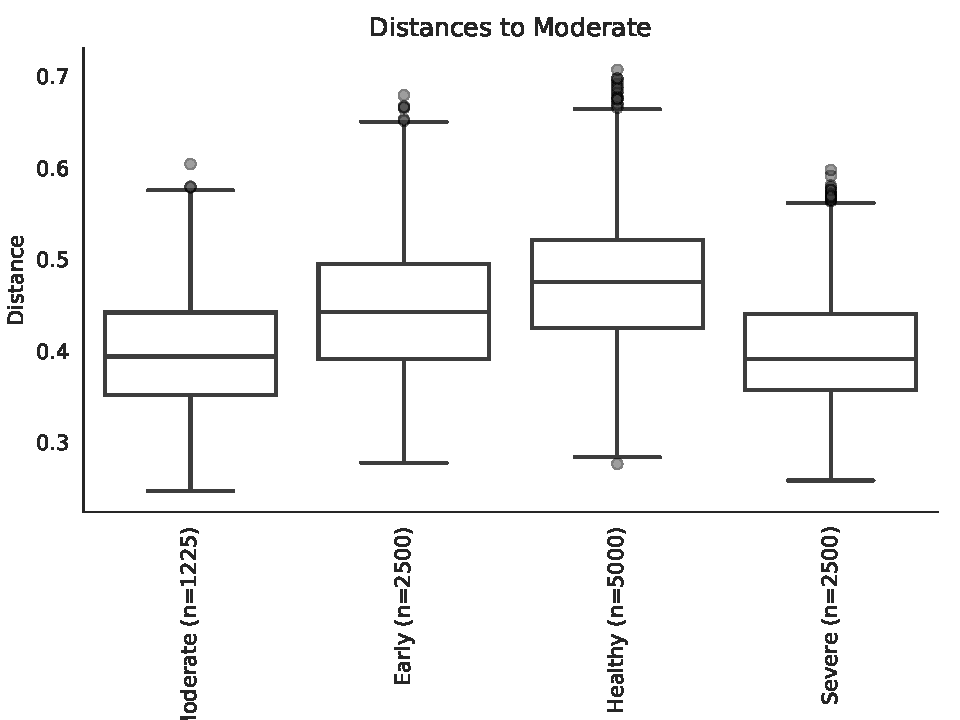
\includegraphics[width=0.4 \linewidth]{figures/BetaDiversity/Deblur/UnweightedUnifrac/Moderate.pdf}
                    &
                    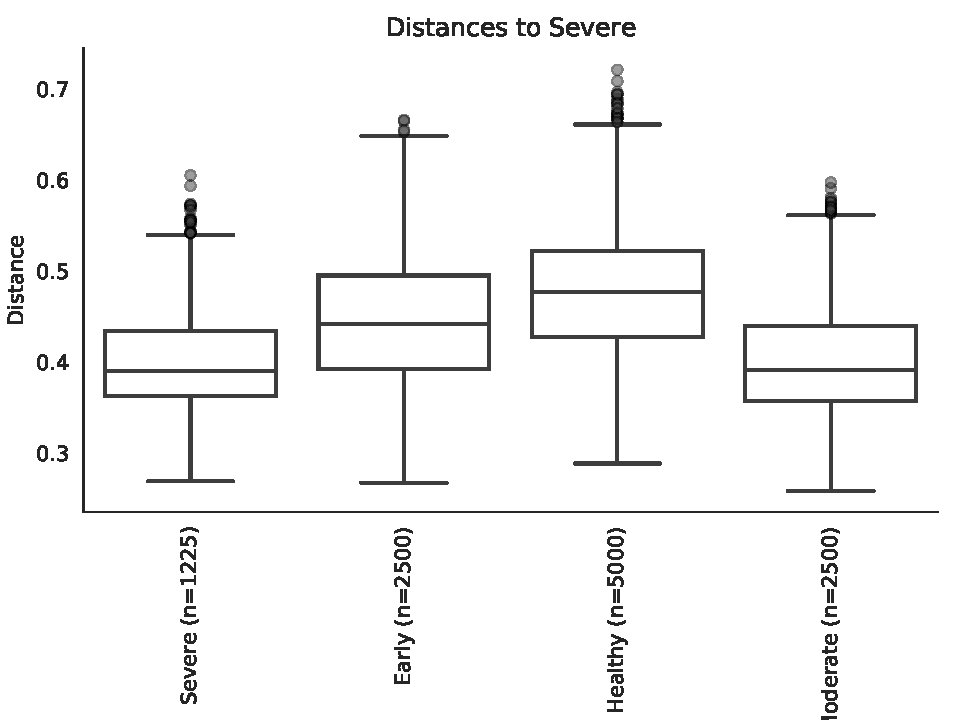
\includegraphics[width=0.4 \linewidth]{figures/BetaDiversity/Deblur/UnweightedUnifrac/Severe.pdf}
                    \\
                    \mbox{(c) Moderate} & \mbox{(d) Severe} \\
                \end{array}$
                \caption{Unweighted Unifrac Distance Index with Deblur}
                \label{fig:unweighted-deblur}
            \end{figure}

            \begin{figure}[p]
                \centering
                $\begin{array}{cc}
                    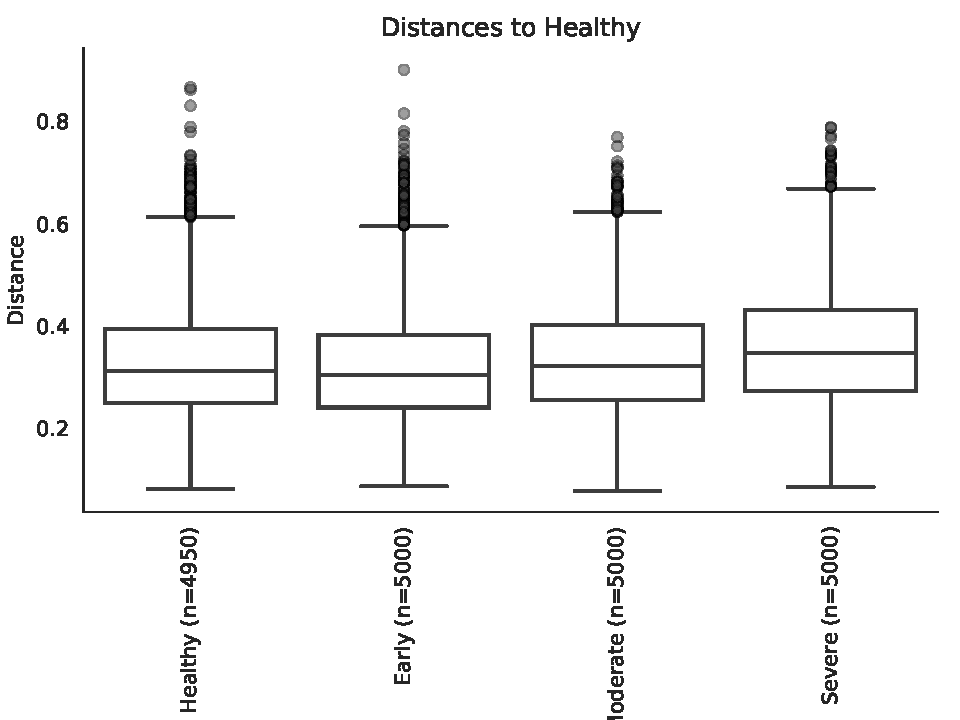
\includegraphics[width=0.4 \linewidth]{figures/BetaDiversity/Deblur/WeightedUnifrac/Healthy.pdf}
                    &
                    \includegraphics[width=0.4 \linewidth]{figures/BetaDiversity/Deblur/WeightedUnifrac/Early.pdf}
                    \\
                    \mbox{(a) Healthy} & \mbox{(b) Early} \\

                    \includegraphics[width=0.4 \linewidth]{figures/BetaDiversity/Deblur/WeightedUnifrac/Moderate.pdf}
                    &
                    \includegraphics[width=0.4 \linewidth]{figures/BetaDiversity/Deblur/WeightedUnifrac/Severe.pdf}
                    \\
                    \mbox{(c) Moderate} & \mbox{(d) Severe} \\
                \end{array}$
                \caption{Weighted Unifrac Distance Index with Deblur}
                \label{fig:weighted-deblur}
            \end{figure}

        \subsection{ANCOM}
            Statistically significant different taxa and volcano plots by ANCOM were derived: DADA2 and Greengenes (Table \ref{tb:ANCOM-dada2-gg} and Figure \ref{fig:volcano-dada2-gg}), DADA2 and SILVA (Table \ref{tb:ANCOM-dada2-silva} and Figure \ref{fig:volcano-dada2-silva}), Deblur and Greengenes (Table \ref{tb:ANCOM-deblur-gg} and Figure \ref{fig:volcano-deblur-gg}) and Deblur and SILVA (Table \ref{tb:ANCOM-deblur-silva} and Figure \ref{fig:volcano-deblur-silva}).

            \begin{table}[p]
                \centering
                \caption{ANCOM Significant Taxa with DADA2 and Greengenes}
                \label{tb:ANCOM-dada2-gg}

                \csvreader[tabular=p{10cm}cc, no head, column count=3, table head=\hline, late after first line=\\\hline, table foot=\hline, respect underscore]{csv/ANCOM/DADA2.gg.csv}{}{\csvlinetotablerow}
            \end{table}

            \begin{figure}[p]
                \centering
                \includegraphics[width=0.8 \linewidth]{figures/ANCOM/DADA2.gg.png}
                \caption{ANCOM Volcano Plot with DADA2 and Greengenes}
                \label{fig:volcano-dada2-gg}
            \end{figure}

            \begin{table}[p]
                \centering
                \caption{ANCOM Significant Taxa with DADA2 and SILVA}
                \label{tb:ANCOM-dada2-silva}

                \csvreader[tabular=p{10cm}cc, no head, column count=3, table head=\hline, late after first line=\\\hline, table foot=\hline, respect underscore]{csv/ANCOM/DADA2.silva.csv}{}{\csvlinetotablerow}
            \end{table}

            \begin{figure}[p]
                \centering
                \includegraphics[width=0.8 \linewidth]{figures/ANCOM/DADA2.silva.png}
                \caption{ANCOM Volcano Plot with DADA2 and SILVA}
                \label{fig:volcano-dada2-silva}
            \end{figure}

            \begin{table}[p]
                \centering
                \caption{ANCOM Significant Taxa with Deblur and Greengenes}
                \label{tb:ANCOM-deblur-gg}

                \csvreader[tabular=p{10cm}cc, no head, column count=3, table head=\hline, late after first line=\\\hline, table foot=\hline, respect underscore]{csv/ANCOM/Deblur.gg.csv}{}{\csvlinetotablerow}
            \end{table}

            \begin{figure}[p]
                \centering
                \includegraphics[width=0.8 \linewidth]{figures/ANCOM/Deblur.gg.png}
                \caption{ANCOM Volcano Plot with Deblur and Greengenes}
                \label{fig:volcano-deblur-gg}
            \end{figure}

            \begin{table}[p]
                \centering
                \caption{ANCOM Significant Taxa with DADA2 and SILVA}
                \label{tb:ANCOM-deblur-silva}

                \csvreader[tabular=p{10cm}cc, no head, column count=3, table head=\hline, late after first line=\\\hline, table foot=\hline, respect underscore]{csv/ANCOM/DADA2.silva.csv}{}{\csvlinetotablerow}
            \end{table}

            \begin{figure}[p]
                \centering
                \includegraphics[width=0.8 \linewidth]{figures/ANCOM/Deblur.silva.png}
                \caption{ANCOM Volcano Plot with Deblur and SILVA}
                \label{fig:volcano-deblur-silva}
            \end{figure}

        \subsection{t-SNE Plot with Whole Microbiome}
            As mentioned herein-before, t-SNE is a technique which reduce multi-dimensional data into two-dimension. Whole microbiome data are multi-dimensional data, which have \textit{circa} 600 columns, so the data should be reduced their dimension for readability. Hence, by the grace of t-SNE, the microbiome data have been deflated their dimension: 328 taxa from DADA2 and Greengenes (Figure \ref{fig:tsne-whole-dada2-gg}), 633 taxa from DADA2 and SILVA (Figure \ref{fig:tsne-whole-dada2-silva}), 232 taxa from Deblur and Greengenes (Figure \ref{fig:tsne-whole-deblur-gg}) and 414 taxa from Deblur and SILVA (Figure \ref{fig:tsne-whole-deblur-silva}).

            \begin{figure}[p]
                \centering
                \includegraphics[width=0.6 \linewidth]{figures/tSNE/Whole/whole.DADA2.gg.png}
                \caption{t-SNE Plot with Whole Microbiome from DADA2 and Greengenes}
                \label{fig:tsne-whole-dada2-gg}
            \end{figure}

            \begin{figure}[p]
                \centering
                \includegraphics[width=0.6 \linewidth]{figures/tSNE/Whole/whole.DADA2.silva.png}
                \caption{t-SNE Plot with Whole Microbiome from DADA2 and SILVA}
                \label{fig:tsne-whole-dada2-silva}
            \end{figure}

            \begin{figure}[p]
                \centering
                \includegraphics[width=0.6 \linewidth]{figures/tSNE/Whole/whole.Deblur.gg.png}
                \caption{t-SNE Plot with Whole Microbiome from Deblur and Greengenes}
                \label{fig:tsne-whole-deblur-gg}
            \end{figure}

            \begin{figure}[p]
                \centering
                \includegraphics[width=0.6 \linewidth]{figures/tSNE/Whole/whole.Deblur.silva.png}
                \caption{t-SNE Plot with Whole Microbiome from Deblur and SILVA}
                \label{fig:tsne-whole-deblur-silva}
            \end{figure}

        \subsection{t-SNE Plot with ANCOM Selected Microbiome Data}
            As whole microbiome data, ANCOM selected microbiome data are also multi-dimensional data, even though their columns are selected by ANCOM. Hence, with t-SNE, ANCOM selected microbiome data have also been deflated their dimension: 15 taxa (as Table \ref{tb:ANCOM-dada2-gg}) from DADA2 and Greengenes (Figure \ref{fig:tsne-ANCOM-dada2-gg}), 23 taxa (as Table \ref{tb:ANCOM-dada2-silva}) from DADA2 and SILVA (Figure \ref{fig:tsne-ANCOM-dada2-silva}), 27 taxa (as Table \ref{tb:ANCOM-deblur-gg}) from Deblur and Greengenes (Figure \ref{fig:tsne-whole-deblur-gg}) and 20 taxa (as Table \ref{tb:ANCOM-deblur-silva}) from Deblur and SILVA (Figure \ref{fig:tsne-ANCOM-deblur-silva}).

            \begin{figure}[p]
                \centering
                \includegraphics[width=0.6 \linewidth]{figures/tSNE/ANCOM/ANCOM.DADA2.gg.png}
                \caption{t-SNE Plot with ANCOM Selected Microbiome Data from DADA2 and Greengenes}
                \label{fig:tsne-ANCOM-dada2-gg}
            \end{figure}

            \begin{figure}[p]
                \centering
                \includegraphics[width=0.6 \linewidth]{figures/tSNE/ANCOM/ANCOM.DADA2.silva.png}
                \caption{t-SNE Plot with ANCOM Selected Microbiome Data from DADA2 and SILVA}
                \label{fig:tsne-ANCOM-dada2-silva}
            \end{figure}

            \begin{figure}[p]
                \centering
                \includegraphics[width=0.6 \linewidth]{figures/tSNE/ANCOM/ANCOM.Deblur.gg.png}
                \caption{t-SNE Plot with ANCOM Selected Microbiome Data from Deblur and Greengenes}
                \label{fig:tsne-ANCOM-deblur-gg}
            \end{figure}

            \begin{figure}[p]
                \centering
                \includegraphics[width=0.6 \linewidth]{figures/tSNE/ANCOM/ANCOM.Deblur.silva.png}
                \caption{t-SNE Plot with ANCOM Selected Microbiome Data from Deblur and SILVA}
                \label{fig:tsne-ANCOM-deblur-silva}
            \end{figure}

        \subsection{Random Forest Classifier with Every Class}

            \begin{table}[p]
                \centering
                \caption{Taxa with DADA2 and GreenGeenes Ordered by Random Forest}
                \label{tb:RF-whole-dada2-gg}

                \csvreader[tabular=cp{10cm}l, no head, column count=3, table head=\hline, late after first line=\\\hline, table foot=\hline]{csv/RandomForest/whole-DADA2-gg.txt}{}{\csvlinetotablerow}
            \end{table}

            \begin{table}[p]
                \centering
                \caption{Taxa with DADA2 and GreenGeenes Ordered by Random Forest}
                \label{tb:RF-whole-dada2-silva}

                \csvreader[tabular=cp{10cm}l, no head, column count=3, table head=\hline, late after first line=\\\hline, table foot=\hline]{csv/RandomForest/whole-DADA2-silva.txt}{}{\csvlinetotablerow}
            \end{table}

            \begin{table}[p]
                \centering
                \caption{Taxa with DADA2 and GreenGeenes Ordered by Random Forest}
                \label{tb:RF-whole-deblur-gg}

                \csvreader[tabular=cp{10cm}l, no head, column count=3, table head=\hline, late after first line=\\\hline, table foot=\hline]{csv/RandomForest/whole-Deblur-gg.txt}{}{\csvlinetotablerow}
            \end{table}

            \begin{table}[p]
                \centering
                \caption{Taxa with DADA2 and GreenGeenes Ordered by Random Forest}
                \label{tb:RF-whole-Deblur-silva}

                \csvreader[tabular=cp{10cm}l, no head, column count=3, table head=\hline, late after first line=\\\hline, table foot=\hline]{csv/RandomForest/whole-Deblur-silva.txt}{}{\csvlinetotablerow}
            \end{table}

        \subsection{Random Forest Classifier with Merging (Healthy+Early) Classes}

    \section{Discussion}

    \bibliographystyle{apacite}
    \bibliography{reference}
\end{document}